% Meta-Informationen -------------------------------------------------------
%		Informationen über das Dokument, wie z.B. Titel, Autor, Matrikelnr. etc
%		werden in der Datei _Meta.tex definiert und können danach global
%		verwendet werden.
% --------------------------------------------------------------------------
% Informationen ------------------------------------------------------------
% 	Definition von globalen Parametern, die im gesamten Dokument verwendet
% 	werden können (z.B auf dem Deckblatt etc.).
% --------------------------------------------------------------------------
\newcommand{\titel}{Exposé\\Federated Learning With Individualized Differential Privacy}
\newcommand{\art}{Master's Thesis} %Bachelorarbeit
\newcommand{\ort}{Leipzig}
\newcommand{\hochschule}{Leipzig University}
\newcommand{\fachgebiet}{Database Group}
\newcommand{\fakultaet}{Faculty of Mathematics and Computer Science}
\newcommand{\institut}{Department of Computer Science}
\newcommand{\autor}{Ole Borchardt}
\newcommand{\matrikelnr}{3725924}
\newcommand{\erstbetreuer}{Prof. Dr. Erhard Rahm}
\newcommand{\zweitbetreuer}{XXXXX}
\newcommand{\jahr}{2024}
\newcommand{\invnr}{1337}
\newcommand{\eingereicht}{xx.xx.xxxx}

% Eigene Befehle
\newcommand{\todo}[1]{\textbf{\textsc{\textcolor{red}{(TODO: #1)}}}}

% Autorennamen in small caps
\newcommand{\AutorZ}[1]{\textsc{#1}}
\newcommand{\Autor}[1]{\AutorZ{\citeauthor{#1}}}

% Befehle zur semantischen Auszeichnung von Text
\newcommand{\NeuerBegriff}[1]{\textbf{#1}}
\newcommand{\Fachbegriff}[1]{\textit{#1}}
\newcommand{\Prozess}[1]{\textit{#1}}
\newcommand{\Webservice}[1]{\textit{#1}}
\newcommand{\Eingabe}[1]{\texttt{#1}}
\newcommand{\Code}[1]{\texttt{#1}}
\newcommand{\Datei}[1]{\texttt{#1}}
\newcommand{\Datentyp}[1]{\textsf{#1}}
\newcommand{\XMLElement}[1]{\textsf{#1}}

% Abkürzungen
\newcommand{\vgl}{Vgl.\ }
\newcommand{\ua}{\mbox{u.\,a.\ }}
\newcommand{\zB}{\mbox{z.\,B.\ }}
\newcommand{\bs}{$\backslash$}

% Einfache Anführungszeichen in texttt
\newcommand{\sq}{\textquotesingle}



% Dokumentenkopf -----------------------------------------------------------
% 	Diese Vorlage basiert auf "scrreprt" aus dem koma-script.
%		Die Option draft sollte beim fertigen Dokument ausgeschaltet werden.
% --------------------------------------------------------------------------
\documentclass[
	11pt,					% Schriftgröße
	DIV=10,
	ngerman,				% für Umlaute, Silbentrennung etc.
	a4paper,				% Papierformat
	oneside,				% einseitiges Dokument
	titlepage,				% es wird eine Titelseite verwendet
	parskip=half,			% Abstand zwischen Absätzen (halbe Zeile)
	headings=normal, % Größe der Überschriften verkleinern
	numbers=withendperiod, % Fügt in den Überschriften nach den Zahlen einen Punkt ein
	listof=totoc,				% Verzeichnisse im Inhaltsverzeichnis aufführen
	bibliography=totoc,				% Literaturverzeichnis im Inhaltsverzeichnis aufführen
	index=totoc,				% Index im Inhaltsverzeichnis aufführen
	captions=tableheading,		% Beschriftung von Tabellen oberhalb ausgeben
	final					% Status des Dokuments (final/draft)
]{scrreprt}

\renewcommand*\chapterheadstartvskip{\vspace*{-1.0cm}}

% Bentigte Packages -------------------------------------------------------
%		Weitere Packages, die benötigt werden, sind in die Datei Packages.tex
%		"ausgelagert", um die Vorlage möglichst übersichtlich zu halten.
% --------------------------------------------------------------------------
% Anpassung des Seitenlayouts ----------------------------------------------
% 	siehe Seitenstil.tex
% --------------------------------------------------------------------------
\usepackage[
	automark,			% Kapitelangaben in Kopfzeile automatisch erstellen
	headsepline,	% Trennlinie unter Kopfzeile
	ilines				% Trennlinie linksbündig ausrichten
]{scrlayer-scrpage}
\usepackage{scrhack} % Disable some warnings

\usepackage{pseudocode}
\usepackage{nicefrac}

% Für eine schöne Anordnung von Bildern
%\usepackage{subfigure}

\usepackage{dsfont}
%\usepackage{color}
%
%% Define user colors using the RGB model
%\definecolor{yellow}{rgb}{0.0,1.0,0.0}
%\definecolor{rot}{rgb}{1.0,0.0,0.0}

% Anpassung an Landessprache -----------------------------------------------
% 	Verwendet globale Option german siehe \documentclass
% --------------------------------------------------------------------------
\usepackage[ngerman]{babel}

% Umlaute ------------------------------------------------------------------
% 		Umlaute/Sonderzeichen wie äöüß direkt im Quelltext verwenden (CodePage).
%		Erlaubt automatische Trennung von Worten mit Umlauten.
% --------------------------------------------------------------------------
\usepackage[utf8]{inputenc}
%\usepackage[T1]{fontenc}
%\usepackage{ae} % "schöneres" ä
\usepackage{textcomp} % Euro-Zeichen etc.
\usepackage{lmodern} % schööön

% Grafiken -----------------------------------------------------------------
% 		Einbinden von Grafiken [draft oder final]
% 		Option [draft] bindet Bilder nicht ein - auch globale Option
% --------------------------------------------------------------------------
\usepackage[dvips,final]{graphicx}
\usepackage{wrapfig}
\graphicspath{{Bilder/}} % Dort liegen die Bilder des Dokuments

% Befehle aus AMSTeX für mathematische Symbole z.B. \boldsymbol \mathbb ----
\usepackage{amsmath,amsfonts,amsthm}

% Für Index-Ausgabe; \printindex -------------------------------------------
\usepackage{makeidx}

% Einfache Definition der Zeilenabstände und Seitenränder etc. -------------
\usepackage{setspace}
\usepackage{geometry}

% für gedrehte Tabellen
\usepackage{rotating} 

% Symbolverzeichnis --------------------------------------------------------
% 	Symbolverzeichnisse bequem erstellen, beruht auf MakeIndex.
% 		makeindex.exe %Name%.nlo -s nomencl.ist -o %Name%.nls
% 	erzeugt dann das Verzeichnis. Dieser Befehl kann z.B. im TeXnicCenter
%		als Postprozessor eingetragen werden, damit er nicht ständig manuell
%		ausgeführt werden muss.
%		Die Definitionen sind ausgegliedert in die Datei Abkuerzungen.tex.
% --------------------------------------------------------------------------
\usepackage[intoc]{nomencl}
  \let\abbrev\nomenclature
  \renewcommand{\nomname}{Abkürzungsverzeichnis}
  \setlength{\nomlabelwidth}{.25\hsize}
  \renewcommand{\nomlabel}[1]{#1 \dotfill}
  \setlength{\nomitemsep}{-\parsep}

% Zum Umfließen von Bildern -------------------------------------------------
\usepackage{floatflt}

% Zum Einbinden von Programmcode --------------------------------------------
\usepackage{listings}
\usepackage{xcolor} 
\definecolor{hellgelb}{rgb}{1,1,0.9}
\definecolor{colKeys}{rgb}{0,0,1}
\definecolor{colIdentifier}{rgb}{0,0,0}
\definecolor{colComments}{rgb}{1,0,0}
\definecolor{colString}{rgb}{0,0.5,0}
\lstset{%
    float=hbp,%
    basicstyle=\texttt\small, %
    identifierstyle=\color{colIdentifier}, %
    keywordstyle=\color{colKeys}, %
    stringstyle=\color{colString}, %
    commentstyle=\color{colComments}, %
    columns=flexible, %
    tabsize=2, %
    frame=single, %
    extendedchars=true, %
    showspaces=false, %
    showstringspaces=false, %
    numbers=left, %
    numberstyle=\tiny, %
    breaklines=true, %
    backgroundcolor=\color{hellgelb}, %
    breakautoindent=true, %
%    captionpos=b%
}

% Lange URLs umbrechen etc. -------------------------------------------------
\usepackage{url}


%% Wichtig für korrekte Zitierweise ------------------------------------------

\usepackage[autocite=inline, sorting=none, backend=biber]{biblatex}
\addbibresource{quellen.bib} % Name der .bib-Datei

\usepackage{csquotes} % Empfohlen, um Zitierten Text richtig darzustellen

% ermöglicht Zeilenumbrüche in Captions
\usepackage{caption}


% PDF-Optionen --------------------------------------------------------------
\usepackage[
bookmarks,
bookmarksopen=true,
pdftitle={\titel},
pdfauthor={\autor},
pdfcreator={\autor},
pdfsubject={\titel},
pdfkeywords={\titel},
colorlinks=true,
%linkcolor=red, % einfache interne Verknüpfungen
%anchorcolor=black,% Ankertext
%citecolor=blue, % Verweise auf Literaturverzeichniseinträge im Text
%filecolor=magenta, % Verknüpfungen, die lokale Dateien öffnen
%menucolor=red, % Acrobat-Menüpunkte
%urlcolor=cyan, 
% für die Druckversion können die Farben ausgeschaltet werden:
linkcolor=black, % einfache interne Verknüpfungen
anchorcolor=black,% Ankertext
citecolor=black, % Verweise auf Literaturverzeichniseinträge im Text5
filecolor=black, % Verknüpfungen, die lokale Dateien öffnen
menucolor=black, % Acrobat-Menüpunkte
urlcolor=black, 
%backref,
%pagebackref,
plainpages=false,% zur korrekten Erstellung der Bookmarks
pdfpagelabels,% zur korrekten Erstellung der Bookmarks
hypertexnames=false,% zur korrekten Erstellung der Bookmarks
linktocpage % Seitenzahlen anstatt Text im Inhaltsverzeichnis verlinken
]{hyperref}

% Zum fortlaufenden Durchnummerieren der Fußnoten ---------------------------
\usepackage{chngcntr}


% für lange Tabellen
\usepackage{longtable}
\usepackage{array}
\usepackage{ragged2e}
\usepackage{lscape}

\usepackage{supertabular}

% Spaltendefinition rechtsbündig mit definierter Breite ---------------------
\newcolumntype{w}[1]{>{\raggedleft\hspace{0pt}}p{#1}}

% Formatierung von Listen ändern
\usepackage{paralist}
% Standardeinstellungen:
% \setdefaultleftmargin{2.5em}{2.2em}{1.87em}{1.7em}{1em}{1em}

\usepackage{tablefootnote}
% für Ausblenden der Seitenzahl
\usepackage{lipsum}

% für subfigures
\usepackage{caption}
\usepackage{subcaption}

% für Durchschnittszeichen
\usepackage{wasysym}

% für tabellen
\usepackage{multirow}

% Erstellung eines Index und Abkürzungsverzeichnisses aktivieren -----------
\makeindex
% makeindex Masterarbeit.nlo -s nomencl.ist -o Masterarbeit.nls
\makenomenclature


% Kopf- und Fußzeilen, Seitenränder etc. -----------------------------------
% Zeilenabstand ------------------------------------------------------------
\onehalfspacing 
% \setstretch{1,5}

% Seitenränder -------------------------------------------------------------
\geometry{paper=a4paper,left=25mm,right=20mm,top=20mm, bottom=25mm}
% Notfall maße :)
%\geometry{paper=a4paper,left=35mm,right=25mm,top=25mm, bottom=25mm}



% Kopf- und Fußzeilen ------------------------------------------------------
\pagestyle{scrheadings}

% Kopf- und Fußzeile auch auf Kapitelanfangsseiten -------------------------
\renewcommand*{\chapterpagestyle}{scrheadings}

% Schriftform der Kopfzeile ------------------------------------------------
\renewcommand{\headfont}{\normalfont}

% Kopfzeile ----------------------------------------------------------------
\ihead{\textit{\headmark}}
\chead{}
%\ohead{\includegraphics[scale=1]{Bilder/logoKlein.JPG}}
\ohead{}
\setlength{\headheight}{8mm} % Höhe der Kopfzeile
\setheadwidth[0pt]{textwithmarginpar} % Kopfzeile über den Text hinaus verbreitern

% Fußzeile -----------------------------------------------------------------
% \ifoot{\copyright\ \autor \\ \invnr}
% \ifoot{\copyright\ \autor \\ \matrikelnr}
\ifoot{\autor \\ \matrikelnr}
\cfoot{}
\ofoot{\pagemark}
\setlength{\footskip}{12mm}
\setfootwidth[0pt]{text}

% Überschriften ------------------------------------------------------------
\renewcommand*\chapterheadstartvskip{\vspace*{-0.5cm}} % Platz vor einer Überschrift eines neuen Kapitels


% erzeugt ein wenig mehr Platz hinter einem Punkt --------------------------
\frenchspacing

% Schusterjungen und Hurenkinder vermeiden
\clubpenalty = 10000
\widowpenalty = 10000 
\displaywidowpenalty = 10000


% Quellcode-Ausgabe formatieren --------------------------------------------
%\lstset{numbers=left, numberstyle=\tiny, numbersep=5pt, breaklines=true}
%\lstset{emph={square}, emphstyle=\color{red}, emph={[2]root,base}, emphstyle={[2]\color{blue}}}

\definecolor{gray}{rgb}{0.9,0.9,0.9}

\lstset{%
		basicstyle=\small\ttfamily,language={[LaTeX]TeX},
		numbersep=5mm, 
		numbers=left,
		numberstyle=\tiny,
		breaklines=true,
		framexleftmargin=8mm, 
		xleftmargin=8mm,
		backgroundcolor=\color{gray},
		captionpos=b
}%

% Fußnoten fortlaufend durchnummerieren ------------------------------------
\counterwithout{footnote}{chapter}

% Definitionen

\newtheorem{definition}{Definition}


% Eigene Definitionen für Silbentrennung
\hyphenation{Trenn-bar-es}
\hyphenation{Al-go-rith-mus}
\hyphenation{DP-Al-go-rith-men}
% Das eigentliche Dokument -------------------------------------------------
%		Der eigentliche Inhalt des Dokuments beginnt hier. Die einzelnen Seiten
%		und Kapitel werden in eigene Dateien ausgelagert und hier nur inkludiert.
% --------------------------------------------------------------------------

\begin{document}
% auch subsubsection nummerieren
\setcounter{secnumdepth}{3}
\setcounter{tocdepth}{3}

% keine Kopf-/Fußzeilen bei Deckblatt und Abstract
\ofoot{}
% Deckblatt
\thispagestyle{plain}
\begin{titlepage}

\begin{center}

\includegraphics[height=7cm]{Bilder/Uni-L.png}\\[2.5ex]

\institut\\
\fakultaet\\
\fachgebiet\\[6ex]

\textbf{\large\titel}\\[1.5ex]
\art\\[6ex]

\normalsize
vorgelegt von:\\
\autor\\[1.5ex]
Matrikelnummer:\\
\matrikelnr\\[1.5ex]
Betreuer:\\
\erstbetreuer\\
\zweitbetreuer\\[1.0ex]
\end{center}

%\begin{tabbing}
%\hspace{3.5cm}\= \kill
%   vorgelegt von: \> \autor\\[1.2ex]
%   Matrikelnummer: \> \matrikelnr\\[1.2ex]
%    \> \\
%   Betreuer: \> \erstbetreuer\\[1.2ex]
%    \> \zweitbetreuer
%\end{tabbing}

\begin{center}
\copyright\ \jahr\\[1.0ex]
\end{center}

\singlespacing
\small
\noindent Dieses Werk einschließlich seiner Teile ist \textbf{urheberrechtlich geschützt}. Jede Verwertung außerhalb der engen Grenzen des Urheberrechtgesetzes ist ohne Zustimmung des Autors unzulässig und strafbar. Das gilt insbesondere für Vervielfältigungen, Übersetzungen, Mikroverfilmungen sowie die Einspeicherung und Verarbeitung in elektronischen Systemen.

\end{titlepage}


\section*{Zusammenfassung}
\label{sec:Zusammenfassung}

Zusammenfassung meiner Arbeit hier....
% \section*{Danksagung}
\label{sec:Danksagung}
Danksagung
\newpage
\ofoot{\pagemark}

% Seitennummerierung -------------------------------------------------------
%		Vor dem Hauptteil werden die Seiten in großen römischen Ziffern
%		nummeriert...
% --------------------------------------------------------------------------
\pagenumbering{Roman}

\tableofcontents			% Inhaltsverzeichnis

% Abkürzungsverzeichnis ----------------------------------------------------
%\input{Inhalt/Glossar}
%\printnomenclature
%\label{sec:Glossar}

\listoffigures					% Abbildungsverzeichnis
\listoftables					% Tabellenverzeichnis

%\renewcommand{\lstlistlistingname}{Verzeichnis der Listings}
%\lstlistoflistings

% ...danach in normalen arabischen Ziffern ---------------------------------
\clearpage
\pagenumbering{arabic}


% Inhalt -------------------------------------------------------------------
%		Hier können jetzt die einzelnen Kapitel inkludiert werden. Sie müssen
%		in den entsprechenden .TEX-Dateien vorliegen. Die Dateinamen können
% 		natürlich angepasst werden.
% --------------------------------------------------------------------------
\begin{chapter}{Structure}
	\begin{section}{Fundamentals}
		\textbf{Dieser Teil soll Grundlagen beschreiben (es kann ein B.Sc. Informatik vorausgesetzt werden). Es können Arbeiten referenziert werden, die existieren, aber nicht direkt meine Arbeit beeinflusst haben.}
		
		\subsection{Federated Learning}
		\begin{itemize}
			\item 
		\end{itemize}
		
		\subsection{Differential Privacy}
		\begin{itemize}
			\item zunächst beschreiben was Privacy ist und wo sich DP einordnen lässt? (interactive, anstatt non-interactive wie k-anonymity)
			\item Attacken auf Privatheit beschreiben, gegen die DP hilft? (wie in der Introduction von \cite{abadi:2016})
			\item 2006 vorgeschlagen von \cite{dwork:2006}
			\item 
		\end{itemize}
		
		\subsection{Personalized Differential Privacy}
		\begin{itemize}
			\item \cite{alaggan:2016} und \cite{jorgensen:2015} haben Personalized Differential Privacy eingeführt (Alaggan kurz vor Jorgensen)
		\end{itemize}
		
	\end{section}
	
	\begin{section}{Related Work}
		\textbf{Dieser Teil soll Arbeiten referenzieren, die direkt meine Arbeit beeinflusst haben. Dazu zählen auch Arbeiten die die gewählten Parameter rechtfertigen (Verteilung der Budgets, die Budgets selbst, ...)}
		
		\subsection{Wahl der Parameter}
		\subsubsection{Wahl der Privacy-Budgets}
		\begin{itemize}
			\item Wahl zunächst wie bei \cite{boenisch:2023}
			\item \cite{sun:2021} legt Nahe, dass die größe der Budgets um gut trainieren zu können stark von den Datensätzen abhängt
			\begin{itemize}
				\item bei mnist gehen sie von $\epsilon > 0.3$ aus während sie für CIFAR10 erst bei $\epsilon > 5$ sagen, dass ein Großteil der Accuracy beibehalten wird
			\end{itemize}
		\end{itemize}
		\subsubsection{Verteilung der einzelnen Privacy-Gruppen}
		\begin{itemize}
			\item \cite{alaggan:2016} für individual-relaxed Verteilung der Budgets
				\begin{itemize}
					\item auf S.15f beschreiben sie, dass sich die Privacy Einstellungen von Nutzern in 3 Gruppen einteilen lassen (Fundamentalists, Pragmatists und Unconcerned)
					\item \cite{jensen:2005} wird als Beleg für die 0.34, 0.43, 0.23 Verteilung genannt (individual-strict)
					\item \cite{acquisti:2005} ist eine Umfrage, die die weniger strikte Verteilung nahelegt (0.54, 0.37, 0.09) (individual-relaxed)
				\end{itemize}
		\end{itemize}
		
		\subsection{Algorithmus}
		\begin{itemize}
			\item \cite{boenisch:2023} für den Sampling Ansatz
			\item \cite{mcmahan:2016} für FedAvg
			\item \cite{mcmahan:2018} für FedAvg mit DP
			\item \cite{aldaghri:2023} für ein anderes Verfahren mit individualisierter DP im Federated Learning?
			\begin{itemize}
				\item entspricht eher dem Scale Ansatz von \cite{boenisch:2023}
				\item nur mit zwei \glqq{}Privacy Niveaus\grqq{} getestet
			\end{itemize}
		\end{itemize}
		
		\subsection{Ergebnisse anderer Paper auf meinen Datensätzen}
	\end{section}
\end{chapter}
\chapter{Introduction}
%\begin{itemize}
%	\item Angriffe auf FL belegen
%\end{itemize}

Mit der zunehmenden Adaption von KI in vielen alltäglichen Bereichen des Lebens und dem Interesse an repräsentativen Trainingsdaten gewinnt die Frage nach Datensicherheit und dem Schutz der Privatheit der Menschen, die Trainingsdaten für Modelle generieren, immer weiter an Bedeutung. In dem Bereich gewinnen dezentrale Trainingsalgorithmen, die verhindern, dass zum Beispiel auf Smartphones generierte Daten das Gerät verlassen müssen, und mathematisch beweisbare Privatheitsgarantien an Bedeutung.

Differential Privacy hat sich als gute Maßnahme erwiesen, um die Privatheit von einzelnen Nutzern bei einer Vielzahl von Datenauswertungen zu gewährleisten. Die Idee ist, Anfrageergebnisse so zu verändern, dass allgemeine Trends im Ergebnis abgebildet sind, der Einfluss einzelner Datenpunkte jedoch begrenzt wird. Das Konzept ist mathematisch formalisiert und lässt es zu, das Niveau der Privatheit über einen Parameter zu steuern. Es wird seit einigen Jahren auch von großen Firmen in der Privatwirtschaft angewendet. Gerade bei der Auswertung von Monitoring Daten setzen Apple, Google und Uber auf Differential Privacy \parencite{apple:2017, erlingsson:2014, tezapsidis:2017}. 

Beim Training von KI-Modellen auf zentralen Datensätzen gibt es mit dem Differential Privacy Stochastic Gradient Descent (\texttt{DP-SGD}) von \textcite{abadi:2016} ein etabliertes und effizient anwendbares Verfahren. Durch die formal beweisbaren Privatheitsgarantien, kann dies zu mehr Vertrauen bei der Nutzung von Daten geben, die von Menschen generiert werden. Allerdings gibt es besonders sensible Daten, wie zum Beispiel die von Smartphone Tastaturen, von denen ein großer Teil der Nutzer vermutlich nicht will, dass sie ihr Endgerät verlassen.

%Quellen für angriffe auf FL angeben
Um das Training zu ermöglichen ohne eine Zentralisierung der Trainingsdaten erforderlich zu machen, haben \textcite{mcmahan:2016} das \textit{Federated Learning} vorgestellt. Dabei wird \glqq{]die Lernaufgabe durch eine lose Föderation von teilnehmenden Geräten (die wir als Clients bezeichnen) gelöst, die von einem zentralen Server koordiniert werden.\grqq{} \parencite[p.1]{mcmahan:2016} Auch wenn damit das Problem der Zentralisierung von Trainingsdaten gelöst werden kann, ist damit noch nicht die Privatheit der Trainingsdaten gewährleistet, denn Angriffe auf Modellparameter werden nicht verhindert. Um dem Problem zu begegnen wurden Modifikationen des Algorithmus vorgestellt, die für die Clients Differential Privacy Garantien erfüllen \parencite{mcmahan:2018, geyer:2017}.

Auch wenn Differential Privacy beim Training von KI-Modellen die Privatheit der Individuen schützt und gegen einige Angriffe unerlässlich ist, hat sie einen großen Nachteil: Es gibt einen Trade-Off zwischen der Güte der trainierten Modelle und der Privatheit der Trainingsdaten, eine höhere Privatheit verringert die Genauigkeit. Das ist in der Regel bis zu einem Gewissen Grad vernachlässigbar, dennoch gibt es Ideen um diesen Trade-Off effizienter zu machen. 

Da unterschiedliche Menschen unterschiedlich brisante Daten generieren und im Allgemeinen auch verschiedene Anforderungen an ihre Privatheit haben, gibt es Forschung dazu, die Privatheitsgarantien zu individualisieren. So könnten Personen wählen ob sie beispielsweise ein mittleres, hohes oder sehr hohes Privatheitsniveau für ihre Daten möchten. KI-Modelle könnten so während des Trainings mehr aus Daten mit einem kleineren Privatheitsniveau lernen und insgesamt eine bessere Genauigkeit erreichen.

Auch im Federated Learning gibt es Algorithmen, um individuelle Privatheitsgarantien zu nutzen. Allerdings erfordern sie teilweise neu eingeführte Parameter \parencite{shen:2023} oder individualisieren Noise Multiplier \parencite{aldaghri:2023}, was zumindest im zentralisierten Training nicht optimal war \parencite{boenisch:2023}. Dort haben individualisierte Sampling Rates, also die Wahrscheinlichkeit, einen Datenpunkt in einem Trainingsschritt zu nutzen, etwas bessere Ergebnisse geliefert.

In meiner Arbeit liefere ich einen Ansatz, individualisierte Sampling Rates im Federated Learning zu nutzen, um individuelle Privatheitsgarantien für Clients zu gewährleisten. Darüber hinaus gehe ich auch auf Herausforderungen bei der Anwendung von Federated Learning für das Training der Modelle ein. Dazu zählen beispielsweise die Verteilung der Trainingsdaten auf den Clients und der zusätzliche Berechnungsaufwand. Weitere Probleme, die in der Praxis auftreten, werde ich nur erwähnen und beschreiben, da ich das Federated Learning nur simulieren kann. Sie sollten aber unbedingt beachtet werden. Dazu zählen die Heterogenität der Geräte auf denen trainiert wird und die Verfügbarkeit bzw. das Ausfallen der Clients während des Trainings.

In \autoref{chap:fundamentals} beschreibe ich die Grundlagen von Differential Privacy und dem Federated Learning. In \autoref{chap:related-work} beschreibe ich Arbeiten zu individualisierter Differential Privacy und Differential Privacy im Federated Learning. \autoref{chap:methods} beschreibt meinen Algorithmus und zeigt, wie er sich von vorhandenen Arbeiten unterscheidet. Die Experimente, die ich durchgeführt habe und deren Ergebnisse werden in \autoref{chap:experiments} bzw. in \autoref{chap:results} beschrieben.
\chapter{Fundamentals}\label{chap:fundamentals}

%\begin{itemize}
%%	\item evtl Section o.ä. zu Angriffen auf nicht DP-Federated Learning, bzw. warum braucht es DP auch im FL?
%	\item IDP-Teil nach Related Work?
%\end{itemize}

In diesem Kapitel gehe ich auf die Grundlagen ein, die für meine Arbeit wichtig sind. Zunächst gebe ich einen Überblick zu Differential Privacy, beschreibe die zugrundeliegende Idee, formalisiere sie und umreiße die wichtigsten Mechanismen, um sie anzuwenden. Danach beschreibe ich die Grundlagen von Federated Learning, erwähne Probleme, die das Verfahren bei verzerrten Datenverteilungen hat und gehe auf mögliche Privacy Modelle im Federated Learning ein.

\section{Differential Privacy}

%\begin{itemize}
%%	\item Anwendung von DP in the wild (\cite{erlingsson:2014, tezapsidis:2017, apple:2017}) -> steht in introduction
%	\item Randomized Response als anschauliches Beispiel? (ähnlich wie bei \cite[p.1]{erlingsson:2014}) 
%\end{itemize}

Differential Privacy ist ein Verfahren, dass die Privatheit bei interaktiven Anfragen auf Datenbanken schützt. Die zugrundeliegende Datenbank selbst wird dabei nicht verändert, was es von nicht-interaktiven Privatheitsmaßen wie \textit{k-anonymity} abgrenzt. Stattdessen wird die Anfrage an die Datenbank so abgewandelt, dass die Privatheit von Individuen geschützt wird. 

Es wurde von \textcite{dwork:2006} formalisiert, nachdem gezeigt wurde, dass Anforderungen an Privatheit von \textcite{dalenius:1977} in der Praxis nicht umsetzbar sind. In \citeauthor{dalenius:1977} war die Philosophie, dass ein Angreifer nichts lernen soll, was er nicht auch ohne Zugriff auf die Datenbank hätte lernen können. \citeauthor{dwork:2006} zeigt, dass diese Definition aufgrund von Hilfsinformationen, die der Angreifer besitzen kann nicht umsetzbar ist. 

In einem Beispiel von \citeauthor{dwork:2006} gibt es eine Datenbank, aus der die durchschnittliche Größe von litauischen Frauen hervorgeht und die Größe der Individuen eine sensible Information ist. Wenn der Angreifer nun die Hilfsinformation hat \glqq{}Person X ist zwei Zentimeter kleiner als der Durchschnitt litauischer Frauen\grqq{}, dann lernt er die genaue Größe von Person X, unabhängig davon, ob sie in der Datenbank ist oder nicht. 

Stattdessen verfolgt \citeauthor{dwork:2006} mit der Differential Privacy einen Ansatz, bei dem nicht direkt das Wissen des Angreifers einbezogen wird, sondern ob der Angreifer bei einer bestimmten Anfrage mehr über ein Individuum lernen kann, wenn es in der zugrundeliegenden Datenbank ist.

Formal vergleicht Differential Privacy die Wahrscheinlichkeit ein ähnliches Anfrageergebnis zu erhalten, wenn ein Individuum in einer Datenbank ist oder eben nicht. Je näher diese Wahrscheinlichkeiten beieinander liegen, desto weniger kann ein Angreifer durch die Präsenz des Individuums in der Datenbank lernen und desto höher ist die Privatheit. Die Definition aus \cite{dwork:2006} ist folgende:

\begin{definition}\label{def:eps-differential-privacy}
	\emph{\textbf{$\epsilon$-Differential Privacy}} A \textit{randomized mechanism} $\mathcal{M}: \mathcal{D} \rightarrow \mathcal{R}$ with domain $\mathcal{D}$ and range $\mathcal{R}$ satisfies $\epsilon$-differential privacy if for any two adjacent inputs $d$, $d' \in \mathcal{D}$ and for any subset of outputs $S \subseteq \mathcal{R}$ it holds that $$\Pr[\mathcal{M}(d) \in S] \leq e^{\epsilon} \Pr[\mathcal{M}(d') \in S]$$
\end{definition}

Hervorzuheben ist hierbei noch, dass die Definition keine Anforderungen an die Datenbanken $d, d'$ macht, außer, dass sie benachbart sind. Typischerweise gilt dafür die folgende Definition:
% Quelle hinzufügen? Bzw. klar machen warum ich sie hier explizit aufschreibe, nämlich in abgrenzung zu den User-adjacent datasets\cite{mcmahan:2018}
\begin{definition}\label{def:example-adjacency}
	\emph{\textbf{Example-adjacent datasets}} Two datasets $d$ and $d'$ are defined to be example-adjacent if $d'$ can be formed by adding or removing a single example from $d$.
\end{definition}

Wenn in dieser Arbeit von benachbarten Datensätzen die Rede ist, gilt i.A. diese Definition, wenn nicht explizit anders beschrieben.

Eine leicht abgeschwächte Version der Definition fügt einen Parameter $\delta$ hinzu, der die Wahrscheinlichkeit repräsentiert, dass die Privatheitsgarantien nicht eingehalten werden. Er sollte demenstprechend sehr klein gewählt werden.\cite{dwork:2014} Diese Definition ist relevant, da der häufig verwendete Gaussian Mechanism die strengere $\epsilon$-Differential Privacy Definition nicht erfüllt, man aber trotzdem mit ihm arbeiten will. Außerdem ist er für das \textit{Advanced Composition Theorem} notwendig.

\begin{definition}\label{def:eps-delta-differential-privacy}
	\emph{\textbf{$(\epsilon, \delta)$-Differential Privacy}} A \textit{randomized mechanism} $\mathcal{M}: \mathcal{D} \rightarrow \mathcal{R}$ with domain $\mathcal{D}$ and range $\mathcal{R}$ satisfies $(\epsilon, \delta)$-differential privacy if for any two adjacent inputs $d$, $d' \in \mathcal{D}$ and for any subset of outputs $S \subseteq \mathcal{R}$ it holds that $$\Pr[\mathcal{M}(d) \in S] \leq e^{\epsilon} \Pr[\mathcal{M}(d') \in S] + \delta$$
\end{definition}

Darüber hinaus gibt es noch die Rényi-Differential Privacy, die neben dem $\epsilon$ noch einen Parameter $\alpha$ hat. Sie ist für viele Theoreme wichtig, ist aber weniger anschaulich und kann immer in $(\epsilon, \delta)$-Differential Privacy überführt werden, weshalb ich hier nicht weiter auf diese Definition eingehen werde. Es gilt, dass ein Mechanismus, der $(\alpha, \epsilon)$-DP erfüllt auch immer $(\epsilon + \frac{\log 1 / \delta}{\alpha - 1}, \delta)$-DP erfüllt für $0 < \delta < \epsilon$ \cite{mironov:2017}.

Damit eine Anfrage Differential Privacy erfüllt, wird auf ein Anfrageergebnis von $\mathcal{M}$ Rauschen hinzugefügt. Das Rauschen kann beispielsweise aus der Laplace- oder der Normalverteilung gezogen werden. Die Varianz der Verteilung, aus der das Rauschen gezogen wird hängt von der Sensitivität einer Anfrage ab. Sie beschreibt die größtmögliche Veränderung des Anfrageergebnisses, die durch das Hinzufügen oder das Löschen eines Eintrags auftreten kann \cite{dwork:2006}.

\begin{definition}\label{def:l1-sensitivity}
	\emph{\textbf{L1-Sensitivity}} For $\mathcal{M}: \mathcal{D} \rightarrow \mathcal{R}^{d}$, the L1-Sensitivity of $\mathcal{M}$ is 
	$$
	\Delta \mathcal{M} = \max_{d_1, d_2}{||\mathcal{M}(d_1) - \mathcal{M}(d_2)||}_1
	$$
	for all adjacent datasets $d_1$, $d_2$
\end{definition}

Die Verteilungen werden je nach Anwendungsfall gewählt. Beispielsweise gibt es den Laplace- oder den Gauss'schen Mechanismus, um numerische Anfragen, beispielsweise Durchschnitt einer Datenbank, privat zu machen. Für Anfragen, die ein Ergebnis aus einer festgelegten Menge liefern sollen, gibt es den Exponentiellen Mechanismus. Dieser bewertet die potenziellen Ergebnisse anhand einer Bewertungsfunktion.\cite{mcsherry:2007}

Bei den Mechanismen ist variiert die Definition der Sensitivität leicht, beispielsweise nutzt der Gauss'sche Mechanismus die $\ell_2$-Norm anstatt der $\ell_1$-Norm, die Intuition, dass es um die maximale Abweichung im Anfrageergebnis durch ein Individuum geht, bleibt jedoch immer erhalten. Darüber hinaus erfüllt der Laplace Mechanismus $\epsilon$-Differential Privacy, der Gauss'sche Mechanismus jedoch nur $(\epsilon, \delta)$-Differential Privacy.\cite[p.261ff]{dwork:2014}

Mit den bisher erwähnten Methoden kann die Privatheit einzelner Anfragen gewährleistet werden. Wenn aber mehrfach Anfragen gestellt werden, muss auch das Niveau der Privatheit abnehmen, da der Durchschnitt der einzelnen Anfragen irgendwann gegen den echten Wert konvergiert \cite[p.42]{dwork:2014}. Ein großer Vorteil von Differential Privacy ist, dass sich diese Verringerung der Privatheit abschätzen lässt. Dafür gibt es einige Kompositionstheoreme:

Das \textit{Basic Composition Theorem} sagt, dass die $k$-fache Anwendung von jeweils $\epsilon_i$-DP Mechanismen ein Privacy-Budget von $\epsilon = \sum_{i=1}^{k} \epsilon_i$ benötigt. Für die strenge $\epsilon$-DP Defintion ist das die optimale Abschätzung \cite{steinke:2022}. Allerdings wächst damit das Privacy Budget linear mit der Anzahl der Anfragen. 

Das Theorem lässt sich auch auf $(\epsilon, \delta)$-DP übertragen, allerdings gibt es dafür mit dem \textit{Advanced Composition Theorem} auch eine asymptotisch bessere Abschätzung. Details dazu sind in \textcite{dwork:2010, steinke:2022} zu finden.

Mechanismen, bei denen ein Subsampling durchgeführt wird, also bei denen nur eine zufällige Teilmenge der Datenbank ausgewertet wird können weitere Privacy Vorteile mit sich bringen \cite{mironov:2019, steinke:2022}.

Darüber hinaus können Ergebnisse, die durch einen Mechanismus erhalten wurden der Differential Privacy erfüllt, weiterverarbeitet werden, ohne dass die Privatheit weiter kompromittiert wird (\textit{post-processing}) \cite{dwork:2014}.

\subsection{Differential Privacy in Machine Learning}\label{sec:fund-dp-in-ml}

%\begin{itemize}
%%	\item Attacken auf Privatheit beschreiben, gegen die DP hilft? (wie in der Introduction von \cite{abadi:2016})
%%	\item Warum nutzt man DP, was ist die Motivation -> Verteidigung gegen Model Inversion Attacks(?), ...
%	\item was sind Variablen beim Training, die einen Einfluss auf das benötigte Privacy Budget haben? (Da kann dann eine Brücke zum FL geschlagen werden)
%\end{itemize}

Das Ziel von Differential Privacy im Machine Learning, ist es die Privatheit der einzelnen Datenpunkte in den Trainingsdaten zu schützen. Das bezieht sich in dem Fall nicht auf den Schutz der Datenbank, sondern darauf, zu verhindern, dass sensible Informationen aus den Trainingsdaten bei der Nutzung des trainierten Modells durch Dritte gefunden werden können. 

% etwas zu reconstruction attacks
Angriffe auf Machine Learning Modelle sind beispielsweise \textit{Reconstruction Attacks}, \textit{Model Inversion Attacks} oder \textit{Membership Inference Attacks}. Bei \textit{Reconstruction Attacks} wird versucht anhand von Features Originaldaten wiederherzustellen. Auch wenn die meisten Machine Learning Algorithmen Features von Trainingsdaten nicht direkt speichern, gibt es einzelne Algorithmen wie Support Vector Machines die es doch tun und damit diesen Attacken ausgesetzt sein können \cite[p.9ff]{chang:2023}.

Bei \textit{Model Inversion Attacks} wird versucht die Eingabe in ein Modell anhand der Ausgabe vorherzusagen. \textcite{fredrikson:2015} haben APIs von Machine Learning as a Service Anbietern analysiert und eine solche Attacke basierend auf den Antworten ihrer Modelle durchgeführt. Dazu haben sie KI-Modelle trainiert, die sensible Attribute aus Umfragen, aber auch Eingabebilder für eine Gesichtserkennung wiederherstellen konnten. Das hat insbesondere mit den Beispielen gut funktioniert, mit denen die Modelle der Anbieter trainiert wurden und stellt daher ein großes Risiko für Leute dar, die Trainingsdaten zu solchen Modellen beisteuern. Um die Effektivität der Attacke zu minimieren schlagen \citeauthor{fredrikson:2015} vor, den Detailgrad der Ausgabe zu verringern. Sie zeigen, dass das rekonstruierte Bild bei einer Gesichtserkennung deutlich schlechter wird, wenn die Wahrscheinlichkeiten, dass das Bild eine bestimmte Person darstellt, ausreichend gerundet wird. Alternativ kann auf die Ausgabe der Wahrscheinlichkeiten verzichtet werden und nur die wahrscheinlichste Klasse ausgegeben werden.

Insbesondere kann Differential Privacy die Effektivität von \textit{Membership Inference Attacks}\cite{shokri:2017} deutlich verringern \cite[p.14f]{chang:2023}. Das Ziel dieser Attacke ist nicht die Rekonstruktion von Eingabedaten, sondern aufgrund von Ausgaben eines trainierten Modells herauszufinden, ob ein Datenpunkt Teil der Trainingsdaten war.

Im Allgemeinen entsteht durch die Anwendung von Differential Privacy im Machine Learning ein Trade-Off zwischen der Nützlichkeit und der Privatheit des Modells (\textit{Privacy-Utility Trade-off}). Daher wird auf verschiedene Arten versucht dabei eine möglichst gute Nützlichkeit des Modells beizubehalten. Zum einen wird an besseren Abschätzungen der Privacy-Kosten geforscht \cite{dwork:2010, abadi:2016, mironov:2019}. Darüber hinaus werden Algorithmen entwickelt, die bessere Ergebnisse erzielen können als andere \cite{papernot:2017}. Es gibt auch Arbeiten, die sich mit der Modellarchitektur selbst beschäftigen, z.B. haben \textcite{papernot:2021} den Effekt von Aktivierungsfunktionen auf Privacy Parameter erforscht und konnten mit beschränken Aktivierungsfunktionen neue \textit{State-of-the-art} Genauigkeiten auf MNIST, FashionMNIST und CIFAR10 erzielen.

Eine weitere Forschungsrichtung ist die Anwendung von individuellen Privacy Budgets für einzelne Nutzer oder Datenpunkte. Sie kann sich auf empirische Studien stützen, die nahelegen, dass verschiedene Personen unterschiedliche Anforderungen an die Privatheit ihrer Daten haben \cite{jensen:2005, acquisti:2005}. In \autoref{fund-idp} und den weiteren Kapiteln werde ich diese Forschungsrichtung weiter beleuchten.

Im Training selbst gibt es verschiedene Punkte, an denen Differential Privacy ansetzen kann um die Privatheit zu gewährleisten. Jeder Punkt hat verschiedene Vor- und Nachteile, die ich im Folgenden umreiße. Eine Übersicht dazu ist in \autoref{fig:design_principles_dpml} zu sehen.

\begin{figure}[tb]
	\centering
	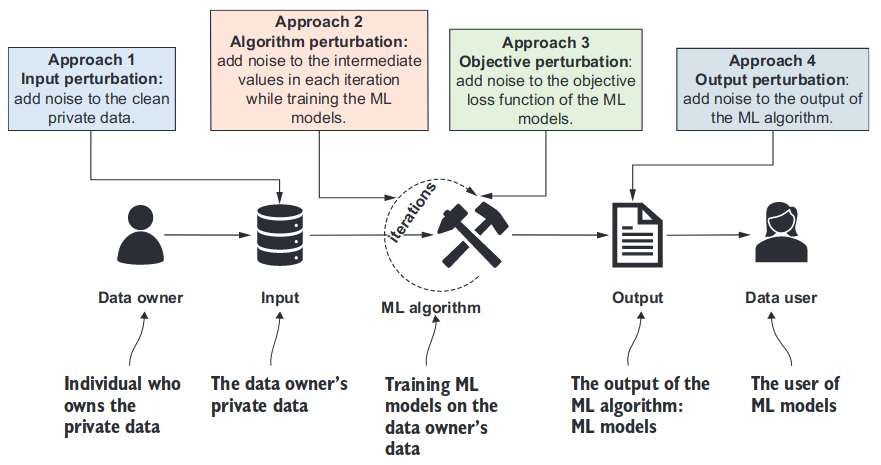
\includegraphics[width=0.9\textwidth]{Bilder/design_principles_dpml.png}
	\caption{Design principles of differentially private ML from \textcite{chang:2023}}
	\label{fig:design_principles_dpml}
\end{figure}

Bei der \textit{Input Pertubation} wird den Trainingsdaten Rauschen hinzugefügt, bevor das Modell mit ihnen trainiert wird. Dieser Ansatz ist ohne weitere Änderungen am Trainingsalgorithmus oder am Modell anwendbar, da der Trainingsalgorithmus dann Daten verarbeitet, die bereits differential private sind und es damit einem \textit{post-processing} entspricht. Das Modell kann danach also problemlos weiterverwendet werden. Ein großer Nachteil ist aber, dass die Anfragen auf den Trainingsdaten im Allgemeinen eine hohe Sensitivität haben und daher viel Rauschen hinzugefügt werden muss.

Die \textit{Algorithm Pertubation} ist das am weitesten verbreitete Verfahren und liegt großen Bibliotheken wie Opacus \cite{yousefpour:2021} und TensorFlow Privacy \cite{tfprivacy} zugrunde. Es kann für iterative Optimierungsverfahren wie Gradient Descent oder die Power Iteration Methode bei einer Principal Component Analysis (PCA) genutzt werden.

Bei der Anwendung dieses Verfahrens im Gradient Descent wird Differential Privacy auf die Gradienten angewendet, das heißt diese werden für gewöhnlich auf eine bestimmte Vektornorm gestutzt und dann wird basierend darauf Rauschen addiert. In der Regel muss hierbei deutlich weniger Rauschen hinzugefügt werden, als bei der \textit{Input Pertubation}.\cite{chang:2023} Der \textit{Privacy Loss}, der durch einen Trainingsdurchlauf anfällt, kann mithilfe von Kompositionstheoremen bestimmt werden. Für die Abschätzung wurde das \textit{Strong Composition Theorem}\cite{dwork:2010} genutzt, allerdings konnten \textcite{abadi:2016} mit dem \textit{Moments Accountant} eine deutlich genauere Abschätzung für das Training von Neuronalen Netzen liefern. So können Neuronale Netze mit dem Verfahren bereits mit kleinen Privacy Budgets trainiert werden. Das trainierte Modell kann ebenfalls veröffentlicht werden, da dessen Gewichte die Anforderungen der Differential Privacy erfüllen. Es schützt also insbesondere nicht nur davor, dass Anfragen an das Modell einem Angreifer Informationen geben können, sondern auch davor dass der Angreifer das Modell herunterlädt und beispielsweise die Modellparameter analysiert.

\textcite{shokri:2015} entwickeln bereits vor \textcite{abadi:2016} ein dezentrales Trainingsverfahren für Neuronale Netze unter Einhaltung von Differential Privacy. Ähnlich wie im Federated Learning (siehe \autoref{fund-fl}) schlagen sie ein verteiltes Training vor. In ihrem Protokoll werden von jedem Teilnehmer nur eine Teilmenge seiner Parameter geteilt, weshalb die Privacy-Budgets pro Modellparameter spezifiziert werden. Parameter, die einen größeren Gradienten als einen vorher spezifizierten Schwellwert haben, werden mit dem Laplace-Mechanismus verrauscht und dann an den Modell-Server geschickt. Die Summe der Privacy-Budgets für ein ganzes Modell kann allerdings sehr groß werden\cite[p.10]{abadi:2016}.

\textit{Objective Pertubation} verändert die Zielfunktion des Trainings. Statt auf die Daten wird während des Trainings Rauschen auf diese Funktion gelegt.

Bei der \textit{Output Pertubation} wird ein nicht-privates Modell trainiert und nur die Ausgabe des Modells verrauscht. Dieses Verfahren hat den großen Nachteil, dass es nicht anwendbar ist, wenn das Modell veröffentlicht werden soll.

Ein Vertreter dieses Ansatzes ist \textit{PATE}\cite{papernot:2017}. Hierbei werden \textit{Teacher Models} auf disjunkten Teilmengen der sensitiven Trainingsdaten trainiert. Das Ensemble dieser \textit{Teacher Models} trainiert danach ein \textit{Student Model} auf einem nicht-sensitiven oder öffentlichen Datensatz. Diese Daten müssen nicht gelabelt sein, da die trainierten \textit{Teacher Modelle} die Labels generieren. Vorteil dieses Verfahrens ist, dass es keine Anforderungen an die Modelle oder den Trainingsprozess stellt. Auch die \textit{Teacher Models} müssen nicht privat trainiert werden, denn die Privatheit entsteht dadurch, dass auf die Ausgabe des Ensembles mit dem \textit{Laplace Mechanismus} Rauschen hinzugefügt wird. Das entspricht der \textit{Output Pertubation}. Da die wiederholte Anfrage der \textit{Teacher Modelle} den Verlust an Privacy erhöht, wird nur eine vorher festgelegte Anzahl an ungelabelten Daten für das \textit{Student Model} mit Labels versehen. Dabei wird nur das mit der größten Konfidenz vorhergesagte Label genutzt. So lässt sich der \textit{Privacy Loss} mithilfe von Kompositionstheoremen abschätzen. Das so trainierte \textit{Student Model} hat diese Limitierung nicht und kann veröffentlicht werden.

Abgesehen von der Varianz des Laplaceschen Rauschens ist die Anzahl der \textit{Teacher Models} wichtig für den Trade-Off zwischen Privacy und Genauigkeit. Eine größere Anzahl an \textit{Teacher Models} verringert den Verlust an Privacy, allerdings wird auch deren Genauigkeit verhindert, da die Menge der Trainingsdaten pro \textit{Teacher Model} abnimmt.

\textcite{papernot:2017} evaluieren \textit{PATE} auf MNIST und SVHN. Im Fall von SVHN nutzen sie die \textit{Extended Version} des Datensatzes und betonen, dass die größere verfügbare Menge an Trainingsdaten die zusätzliche Komplexität des Datensatzes kompensiert. Mit 250 \textit{Teacher Models} können sie Genauigkeiten von $98\%$ (MNIST) und $90.66\%$ (SVHN) erzielen. Das Ergebnis auf MNIST kann damit \textcite{abadi:2016} schlagen.

Der größte Nachteil an PATE ist, dass der Algorithmus nicht-private (potenziell ungelabelte) Daten benötigt, da das \textit{Student Model} nicht-privat trainiert wird. Diese Voraussetzung braucht der Algorithmus von \textcite{abadi:2016} nicht.

\subsection{Individualized Differential Privacy}\label{fund-idp}

Motiviert von den verschiedenen Anforderungen und Präferenzen unterschiedlicher Personen an die Privatheit ihrer Daten haben \textcite{alaggan:2016} und wenig später unabhängig \textcite{jorgensen:2015} Arbeiten zu Differential Privacy mit individuellen Privacy Budgets veröffentlicht.

\textcite{alaggan:2016} definieren heterogene Differential Privacy im Kontext von Nutzerprofilen. In ihrer Arbeit individualisieren sie die Privacy durch das Anpassen der Sensitivität der Komponenten mit unterschiedlichen Budgets. Dazu erstellen sie eine \textit{Shrinkage Matrix}, mit der die Datenpunkte multipliziert werden. Die Matrix ist eine Diagonalmatrix, bei der die Diagonalelemente in $[0;1]$ liegen und abhängig von dem jeweiligen Privacy-Budget sind.

Ihr Ansatz ist jedoch für einige Funktionen nicht anwendbar, beispielsweise können das Minimum und die $\ell_0$-Norm nicht berechnet werden.

\textcite{jorgensen:2015} stellen einen Sampling Ansatz vor, mit dem beliebige DP-Algorithmen in einen Algorithmus mit individualisierter DP überführt werden können. Dabei wird der zugrundeliegende DP-Algorithmus als Black Box betrachtet und die Wahrscheinlichkeit, dass ein Tupel für den Algorithmus gezogen wird, davon abhängig gemacht, was der Nutzer als Privacy Budget gewählt hat.

In ihren Experimenten betrachten sie das gewählte Privacy Budget eines Nutzers als öffentliche Information. Dies kann als problematisch gewertet werden, da es theoretisch etwas über die Wichtigkeit einer Information aussagen kann. Sie rechtfertigen diesen Umstand damit, dass die Budgets nicht für ein Attribut gewählt werden sondern für ein Individuum mit potenziell vielen Attributen und diese Information daher nur etwas über die Person aussagt. Darüber hinaus plädieren sie dafür, einen Nutzer anstatt eines genauen Budgets eine bestimmte Privatheitsstufe mit angemessener Beschreibung (niedrig, mittel und hoch) zu spezifizieren, damit die Semantik der Budgets für Endnutzer verständlich bleibt.

Darüber hinaus zeigen sie ein weiteres Verfahren basierend auf dem \textit{Exponential Mechanism}. Diesen verändern sie dazu so, dass die Score-Funktion die individuellen Privacy Budgets mitbetrachtet. Sie wenden diesen Mechanismus auf \textit{Count}, \textit{Median} und \textit{Min} an, merken aber an, dass das Finden eines Algorithmus, der die angepasste Score-Funktion für beliebige Funktionen effizient berechnet, nicht trivial ist.

Sie weisen die Effektivität ihrer Verfahren in Experimenten nach, in denen sie beide Verfahren für \textit{Count} und \textit{Median} durchführen und eine \textit{Multiple Linear Regression} mit dem Sampling-Verfahren. Ihre Verfahren vergleichen sie mit Standard-DP Verfahren und bei \textit{Count} zusätzlich mit den Stretching-Verfahren aus \cite{alaggan:2016}. Die Privacy Budgets teilen sie in drei Gruppen mit aufsteigenden Privacy-Budgets auf (\textit{conservative}, \textit{moderate} und \textit{liberal}). Bei \textit{Count} leidet das Sampling-Verfahren dadurch, dass Elemente augeschlossen werden. Allerdings kann der angepasste \textit{Exponential Mechanism} gute Ergebnisse liefern und das Stretching-Verfahren deutlich schlagen. \textit{Median} ist verhält sich gegenüber dem Sampling deutlich resistenter, weshalb der Ansatz hier auch gute Ergebnisse erzielen kann und auch besser abschneidet als der modifizierte \textit{Exponential Mechanism}. 

Auch bei der linearen Regression kann der Sampling Ansatz das Verfahren von \cite{alaggan:2016} schlagen. Der modifizierte \textit{Exponential Mechanism} ist hier nicht anwendbar.

\section{Federated Learning}\label{fund-fl}

Federated Learning (FL) ist ein Optimierungsverfahren, bei dem einzelne Clients gemeinsam über mehrere Runden ein Modell trainieren, ohne dabei ihre eigenen Trainingsdaten mit anderen zu teilen. Auch wenn noch viele Fragen im Federated Learning offen sind und erforscht werden, wird es erfolgreich in Produktivumgebungen eingesetzt und stellt im Training mit besonders sensiblen Daten eine gute Alternative gegenüber dem klassischen zentralisierten Training dar \cite{hard:2018, ramaswamy:2020}.

Im Federated Learning gibt es einen Server, der den Ablauf des Trainings steuert und eine beliebige Anzahl von Clients, die das lokale Training auf ihren eigenen Daten durchführen. Der generelle Ablauf einer Trainingsrunde sieht wie folgt aus: 

\begin{enumerate}
	\item der Server initialisiert ein Modell und dessen Parameter (nur erste Runde) 
	\item \label{round-start} er wählt eine Menge von Clients aus, mit denen in dieser Runde das Modell trainiert werden soll
	\item das Modell wird an die ausgewählten Clients geschickt
	\item die Clients optimieren das Modell auf ihren eigenen Daten und schicken die aktualisierten Parameter zurück an den Server
	\item der Server aggregiert die Parameter der Clients und konstruiert daraus neue Modellparameter
	\item danach geht es in der nächsten Runde mit \autoref{round-start} weiter bis das Modell konvergiert oder die festgelegte Rundenzahl erreicht ist
\end{enumerate}

Die lokale Optimierung und die Aggregation der Updates variiert je nach Algorithmus. Die beiden Standardalgorithmen sind \texttt{FedAvg} und \texttt{FedSGD}\cite{mcmahan:2016}. Der wichtigste Unterschied ist, dass \texttt{FedAVG} die Clients mehrere Epochen auf ihren eigenen Daten trainieren lässt, während die Clients im \texttt{FedSGD} nur einen Schritt machen, bevor sie die aktualisierten Parameter wieder an den Server schicken. In beiden Algorithmen werden die Updates bei der Aggregation nach der Menge an Datenpunkten beim jeweiligen Client gewichtet.

Das verteilte Training kann vor allem zwei Probleme mit sich bringen: Zunächst kann der Zusatzaufwand für die Kommunikation sehr groß werden, gerade wenn über viele Runden hinweg trainiert wird. Zum anderen kann nicht angenommen werden, dass die Daten über die Clients hinweg unabhängig und gleichverteilt (i.i.d.) sind, was die Konvergenz der Algorithmen beeinträchtigen kann. \textcite{karimireddy:2020} versuchen diesem Problem zu begegnen, indem sie in ihrem Algorithmus die generelle Richtung, in die die Clients optimieren, an die Clients schicken und diese sie in ihre Updates einfließen lassen.

Die Anwendungsfälle von Federated Learning können variieren: Zum einen gibt es das \textit{Cross-device Federated Learning} und zum anderen das \textit{Cross-silo Federated Learning}\cite{kairouz:2021}. 

Ersteres entspricht dem Fall, dass die Clients eine Vielzahl von mobilen oder IoT-Geräten sind. Hierbei sind die Clients sehr unzuverlässig, zum Beispiel kann der Empfang zu schlecht werden, ein Gerät ausgeschaltet werden oder wegen einem zu niedrigen Akkustand ungeeignet für die Teilnahme am Training sein. All dies kann von dem Server nicht beeinflusst werden, also muss das Trainingsverfahren mit solchen Ausfällen zurecht kommen. Darüber hinaus kann die Menge der Clients von dem Server nicht verlässlich indiziert werden, da Geräte auch dauerhaft ausfallen können, zum Beispiel wenn ein Mobiltelefon kaputt geht oder ein neues gekauft wird und deshalb laufend neue Geräte hinzukommen können.

Bei dem \textit{Cross-silo Federated Learning} geht es vor allem um das Trainieren von Modellen zwischen unterschiedlichen Datencentern oder Organisationen. Die Motivation hierbei ist vor allem, dass es ein gemeinsames Interesse mehrerer Parteien an aussagekräftigen Modellen gibt, die zugrundeliegenden Trainingsdaten aber nicht den anderen Organisationen bereitgestellt werden sollen. Hierbei ist die Ausfallsicherheit der Clients deutlich höher als beim \textit{Cross-device Federated Learning} und auch die Menge der Clients ist in der Regel bekannt.

Auch der Server selbst kann bei einer sehr großen Zahl an Clients zu einem Bottleneck werden.\cite[p.11]{kairouz:2021} Daher wird ebenfalls an vollständig verteilten Trainingsverfahren geforscht, bei denen kein zentraler Server nötig ist (\textit{Fully-decentralized learning}).

\subsection{Data heterogeneity}\label{fund-fl-data-heterogenity}

Ein häufig beschriebenes Problem des Federated Learnings ist die Heterogenität der Trainingsdaten. Da die Daten von unterschiedlichen Parteien generiert werden ist eine zufällige Verteilung der abhängigen und unabhängigen Variablen in der Regel nicht gegeben. Diese Heterogenität kann sich auf verschiedene Arten ausdrücken, wie im folgenden beschrieben.

Die Daten auf den einzelnen Clients können Abhängigkeiten aufweisen, beispielsweise wenn sie in einer zeitlichen Abfolge sortiert vorliegen. Derartige Abhängigkeiten können aber durch das Durchmischen der einzelnen Datenpunkte gelöst werden. Eine solche Verzerrung wird \textit{Intra-Client Distribution Skew} genannt.

Die Verteilung der Features kann sich zwischen den Clients unterscheiden, auch wenn die Wahrscheinlichkeit der Labels gegeben der Features, $P(y|x)$, die gleiche ist. Beispielsweise könnte es sein, dass eine Person sehr viele Hundebilder auf ihrem Handy hat, weil sie ein Hund als Haustier hat und eine andere Person sehr viele Katzenbilder, weil sie mit einer Katze wohnt. Diese Art von Verzerrung heißt \textit{Feature Distribution Skew}

Umgekehrt kann sich auch die Verteilung der Labels auf den Clients unterscheiden, zum Beispiel aufgrund von regionalen Unterschieden. Beispielsweise können Kängurus fast nur in Australien beobachtet werden. In diesem Fall wird es als \textit{Label Distribution Skew} bezeichnet.

Darüber hinaus werden von \textcite{kairouz:2021} weitere Verzerrungen erwähnt. So kann es sein, dass sich die bedingten Wahrscheinlichkeiten von Features und Labels unterscheiden, beispielsweise sieht ein Haus in den USA anders aus als in Europa, in beiden Fällen ist es aber ein Haus (\textit{concept drift}). Andersherum kann es auch sein, dass die gleichen Features anders gelabelt sind, beispielsweise weil manche Daten auch für Menschen ununterscheidbar sind. Außerdem kann die Anzahl der Trainingsbeispiele von Client zu Client sehr stark variieren. 

\subsection{Privacy model in Federated Learning}\label{sec:pm-in-fl}
Auch wenn das Training von Modellen im Federated Learning verhindert, dass Trainingsdaten das eigene Gerät verlassen, sind Angriffe auf die trainierten Modelle weiterhin möglich. Das schließt die in \autoref{sec:fund-dp-in-ml} Attacken ein, aber es gibt auch weitere Arbeiten, die sich speziell mit Federated Learning befassen \cite{geiping:2020, wang:2019}. Die Anwendung von Differential Privacy im Federated Learning hat das Potenzial die mit den Attacken verbundenen Risiken zu mindern. Es gibt unterschiedliche Herangehensweisen, um Differential Privacy im Federated Learning umzusetzen.

% local vs global (trusted server), record vs user level
Die bisherige Definition von Differential Privacy geht davon aus, dass die Privatheit einzelner Datenpunkte in einer Datenbank geschützt wird. Im Federated Learning ist die Struktur der Daten eine andere: Es gibt viele Clients und es ist wichtig die Privatheit des ganzen Datensatzes eines Clients zu schützen. Es reicht nicht aus einzelne Zeilen seiner Daten zu schützen. Wenn die Menge der Daten aller Clients als Datenbank angesehen wird, kann die Definition der benachbarten Datensätze aus  \autoref{def:example-adjacency} dementsprechend angepasst werden:

\begin{definition}\label{def:user-adjacency}
	\emph{\textbf{User-adjacent datasets} \cite{mcmahan:2018}} Let $d$ and $d'$ be two datasets of training examples, where each example is associated with a user. Then, $d$ and $d'$ are \textbf{adjacent} if $d'$ can be formed by adding or removing all of the examples associated with a single user from d.
\end{definition}

Mit dieser Definition kann gewährleistet werden, dass die Anwesenheit oder Abwesenheit der Trainingsdaten eines Nutzers nur einen unmerklichen Einfluss auf die Modellparameter des am Ende vom Lernprozess veröffentlichten Modells hat \cite{mcmahan:2018}.

Darüber hinaus kann Differential Privacy auf zwei Arten angewendet werden: lokal oder global. Bei der globalen Anwendung erfüllt wie oben beschrieben das Modell am Ende Differential Privacy. Allerdings sind die Gradienten, die an den Server geschickt werden nicht privat, denn das nötige Rauschen wird nur auf das Modellupdate angewendet, das aus den Updates aller Clients aggregiert wird. Es muss also dem Server vertraut werden \cite[p.44]{kairouz:2021}.

Alternativ dazu ist die lokale Anwendung von Differential Privacy. Dabei muss das Rauschen hinzugefügt werden, bevor der Client sein Update an den Server schickt. Dem Server wird nicht mehr per se vertraut, stattdessen wird in der Regel angenommen, dass der Server "honest-but-curious" ist. Das bedeutet, dass er zwar die Aufgaben, die er in dem Protokoll hat, richtig umsetzt, aber gleichzeitig versucht, aus den Zwischenergebnissen Informationen zu extrahieren. Auch wenn dieser Ansatz konsequenter ist, hat sich in der Praxis allerdings gezeigt, dass er schwieriger umzusetzen ist, unter anderem, da Zwischenergebnisse stärker verrauscht werden \cite[p.54]{kairouz:2021}.

In meiner Arbeit lege ich den Fokus auf die globale Anwendung von Differential Privacy. In \autoref{chap:related-work} beschreibe ich der Vollständigkeit halber aber auch noch andere Verfahren, die Differential Privacy lokal anwenden.
\chapter{Verwandte Arbeiten}\label{chap:related-work}

%\begin{itemize}
%	%	\item Konvergenz des FL verbessern durch Algorithmen
%	%	\begin{itemize}
%		%		\item Varianz reduzieren (SCAFFOLD), Momente nutzen, ... (sehr viele Ansätze werden in \textcite[p.26ff]{kairouz:2021} erwähnt)
%		%	\end{itemize}
%%	\item Ansätze für personalisierte Modelle (bei non-iid Datensätzen) \parencite[p.28ff]{kairouz:2021} bzw. auch die Idee Globale Modelle durch Kontext anzureichern um bessere Vorhersagen für einzelne Nutzer zu bekommen
%%	\item Ergebnisse von anderen Arbeiten auf den gleichen Datensätzen
%	%	\item Übertragung von non-FL Verfahren auf FL und die Probleme die dabei entstehen (z.B. beim Hyperparametertuning) (p.30ff)
%	%	\item Kompression / Effizienzsteigerung von FL (p.32ff.)
%	%	\item sehr interessanter Absatz zu Kompatibilität von DP und Kompressionstechniken (p.33)
%	%	\item DP in FL (p. 44ff), vor allem die Referenzen zu Hybrid DP tun das was ich machen will aber anders
%	%	\item Kapitel 4.3 (p.48 ff) für mein Szenario mit einem vertrauenswürdigen Server
%	%	\item p.50 hat vieles was bei mir in Future Work kann
%	%	\item p.54 hat ganz klaren Vergleich zwischen Local und Central DP!
%\end{itemize}

In diesem Kapitel beschreibe ich den Stand der Forschung in den für meine Arbeit relevanten Forschungsgebieten. Da sie mehrere Problemfelder umfasst, werde ich das Kapitel im folgenden in drei Teile unterteilen. In \autoref{sec:rw-idp-ml} gehe ich auf Arbeiten ein, die individualisierte Differential Privacy aus \autoref{fund-idp} auf Machine Learning Algorithmen übertragen. In \autoref{sec:rw-fl} beschreibe ich den Stand der Forschung in Bezug auf Fragen des Federated Learning, beispielsweise wie mit unterschiedlichen Verteilungen in den Trainingsdatensätzen umgegangen werden kann. In \autoref{sec:rw-fldp} gehe ich auf Arbeiten ein, welche die Notwendigkeit von Differential Privacy im Federated Learning belegen und auf Algorithmen, welche Differential Privacy mit einheitlichen Privacy-Budgets im Federated Learning umsetzen, um die Basis für Algorithmen mit individualisierten Budgets zu legen, die ich in \autoref{sec:rw-flidp} beschreibe.

\section{Individualisierte Differential Privacy im Machine Learning}\label{sec:rw-idp-ml}

Wie in \autoref{sec:fund-dp-in-ml} angedeutet, ist die Arbeit mit individualisierten Privacy Budgets eine Möglichkeit, die Nützlichkeit eines Machine Learning Modells unter Einhaltung der Privacy Budgets der Nutzer zu erhöhen.

\textcite{boenisch:2023} untersuchen in ihrer Arbeit das Training mit individuellen Privacy Budgets. Sie stellen zwei Verfahren vor: \textbf{SAMPLE} und \textbf{SCALE}. \textbf{SAMPLE} basiert auf \textcite{jorgensen:2015} und erreicht die individuellen Budgets indem Datenpunkte im Training mit unterschiedlichen Wahrscheinlichkeiten gezogen werden. Die Wahrscheinlichkeiten werden etwas anders berechnet als bei \textcite{jorgensen:2015}. \textbf{SCALE} ist inspiriert von \textcite{alaggan:2016}. Anders als bei deren \textit{Stretching Mechanism} werden allerdings nicht die Datenpunkte selbst, sondern das addierte Rauschen skaliert. 

Beide Ansätze werden mit verschiedenen Budgets und Verteilungen der Budgets evaluiert. Sie teilen die Trainingsdaten in drei Gruppen ein (niedriges, mittleres und hohe Privacy Budget). Darüber hinaus testen sie zwei Szenarien, bei denen sich die Größen der drei Gruppen unterscheiden. Die erste Verteilung lässt mehr Trainingspunkte mit hohem und mittleren Budget zu ($34\%$, $43\%$, $23\%$), die andere weniger ($54\%$, $37\%$, $9\%$). Wie bei \textcite{jorgensen:2015} sind die Ergebnisse im ersten Fall besser und werden im zweiten Fall schlechter. In der Evaluation schneidet \textbf{SAMPLE} in allen Experimenten bis auf einem etwas besser ab als \textbf{SCALE}.

Auch für PATE haben \textcite{boenisch:2023b} mit IPATE eine individualisierte Version entwickelt. Sie erforschen zwei unterschiedliche Ansätze: \textit{upsampling} und \textit{weighting}. Der erste dupliziert Datenpunkte in Abhängigkeit von ihrem Privacy-Budget. Damit ist die Disjunktheit der Daten der einzelnen \textit{Teacher Models} nicht mehr gegeben. Mit \textit{weighting} gewichten sie die Stimmen der unterschiedlichen \textit{Teacher Models} unterschiedlich. Sie analysieren die Privacy-Kosten von PATE und IPATE und können mit dem individualisierten Ansatz deutlich mehr Trainingsdaten für das \textit{Student Model} klassifizieren bis die Privacy-Budgets aufgebraucht sind. Außerdem zeigen sie, dass die zusätzlichen Trainingsdaten einen positiven Effekt auf die Genauigkeit des \textit{Student Models} hat.

Die Privacy-Budgets und die Einteilung der Daten in drei Gruppen \citeauthor{boenisch:2023} basieren auf zwei Studien aus dem Jahr 2005 \cite{jensen:2005, acquisti:2005}. Beide untersuchen die Privacy-Präferenzen im Internet. Auch in älteren Studien dazu wird die Einteilung in drei Gruppen vorgenommen, ist also eine gängige Einteilung \cite{westin:1998}.

Bei \textcite{jensen:2005} erfolgt die Einteilung von Befragten basierend auf fünf Fragen. Beantworten sie vier davon mit einem Fokus auf Privatheit, kommen sie in die strengste der drei Gruppen. Beantworten sie keine der Fragen dementsprechend werden sie der Gruppe mit dem größten Privacy Budget zugeordnet. Der Rest kommt in die mittlere Gruppe. So kommen sie auf die Verteilung von ($34\%$, $43\%$, $23\%$) (von strenger zu weniger streng). 

Sie merken an, dass Befragte bei ihren Antworten ihre Sorge um die Privatheit und ihren Willen zu handeln stärker zum Ausdruck bringen, als sie tatsächlich sind. Diese These untermauern sie, indem sie Fragen ob eine Person sich mit Technologien für das Internet-Tracking (Cookies, Web-Bugs, ...) auskennt. Zur Überprüfung haben sie für die Themen Wissensfragen vorbereitet. Nur ein kleiner Teil von den Personen, die angegeben haben sich mit dem Thema auszukennen konnten die Wissensfragen richtig beantworten.

\textcite{acquisti:2005} haben ebenfalls eine Umfrage dazu durchgeführt und bemerken ebenfalls eine Diskrepanz zwischen der Angegebenen Sorge um Privatheit und bisher unternommenen Schritten um diese zu verbessern. Diese Unterschiede in beiden Studien legen Nahe, dass es wichtig ist, den Schutz der Privatheit einfach zu ermöglichen und so zugänglich zu halten, dass die Endnutzer sich nicht weiter mit den Details auskennen müssen. \textcite{jorgensen:2015} plädieren ebenfalls dafür, merken aber an, dass die genaue Wahl eines Privacy-Budgets für ein gegebenes System ein offenes Problem ist.

% noble:2023 Seite 2 für mehr related work!
\section{Federated Learning}\label{sec:rw-fl}

Wie in \autoref{fund-fl} angedeutet, sind \texttt{FedSGD} und vor allem \texttt{FedAvg} die Standardalgorithmen im Federated Learning. Beide sind relativ simpel und in Federated Learning Frameworks wie \textit{tensorflow federated} und \textit{flower} enthalten. In \autoref{alg:fedavg} ist der Pseudocode für \texttt{FedAvg} aus \cite{mcmahan:2016} dargestellt. 


\begin{algorithm}[tb]
	\caption{FederatedAveraging (\texttt{FedAvg})}
	\label{alg:fedavg}
	\SetKwFunction{ClientUpdate}{ClientUpdate}
	\SetKwFunction{Server}{Server}
	\SetKwProg{Fn}{Function}{:}{}
	\Fn{\Server{}}{
		initialize $w_0$; \\
		\For{each round $t = 1, 2, \dots$}{
			$S_t \leftarrow$ random set of $\max(C \cdot K, 1)$ clients\;
			\ForEach{client $k \in S_t$ \textbf{in parallel}}{
				$w_{t+1}^{k} \leftarrow \texttt{ClientUpdate}(k, w_t)$\;
			}
			$w_{t+1} \leftarrow \sum_{k=1}^K \frac{n_k}{n} w_{t+1}^{k}$\;
		}
	}
	\Fn{\ClientUpdate{$k, w$}}{
		\For{each local epoch $i$ from $1$ to $E$}{
			batches $\leftarrow$ data $P_k$ split into batches of size $B$\;
			\For{each batch $b \in$ batches}{
				$w \leftarrow w - \eta \nabla \ell(w; b)$\;
			}
		}
		\KwRet $w$ to server\;
	}
\end{algorithm}

Auch wenn sich der Algorithmus in der Praxis bewährt hat\cite{hard:2018, ramaswamy:2020}, hat er Probleme bei nicht-gleichverteilten Daten. Um die Konvergenz unter solchen Bedingungen zu beschleunigen haben \textcite{karimireddy:2020} und \textcite{li:2020} abgewandelte Algorithmen entworfen.

\textcite{karimireddy:2020} entwickeln \texttt{SCAFFOLD}, einen Algorithmus, der versucht den \textit{client-drift} zu reduzieren, indem die Varianz der Updates durch \textit{control-variates} reduziert wird. \textit{client-drift} beschreibt das Verhalten, dass sich die einzelnen Clients jeweils zu ihrem lokalen Optimum bewegen und der Server zu dem Durchschnitt der Optima. Die Differenz zwischen dem Durchschnitt und dem tatsächlichen globalen Optimum muss bei \texttt{FedAvg} durch kleine Schritte gering gehalten werden wodurch die Konvergenz verlangsamt wird \parencite[p.4]{karimireddy:2020}.

\textcite{li:2020} erlauben den Clients in ihrem Algorithmus \texttt{FedProx} weniger exakte Updates zu erzeugen und fügen der lokalen Verlustfunktion einen \textit{proximal term} hinzu, der gewährleisten soll, dass die lokalen Parameter nicht zu stark von dem globalen Modell abweichen. Der Grund für das Zulassen von weniger exakten Updates ist, dass so weniger potente Clients weniger trainieren können um zu verhindern, dass ihre Ergebnisse aufgrund von Zeitüberschreitungen verworfen werden.

Ein weiteres Problem ist die Wahl geeigneter Hyperparameter für das Training. Da der eigentliche Trainingsprozess in Produktivumgebungen mehrere Tage\cite[p.5]{hard:2018} oder Wochen\cite[p.4]{ramaswamy:2020} dauern kann, ist es in der Regel nicht möglich viele Trainingsdurchläufe durchzuführen. In Verbindung mit Differential Privacy ist das Problem noch verschärft, da bei mehreren Trainingsdurchläufen auch die Privacy Kosten steigen. Damit gibt es dabei ebenfalls einen Trade-Off zwischen Netzwerk- und Ressourcennutzung und guten Hyperparametern. Auch \textcite[p.31]{kairouz:2021} plädieren für mehr Forschung in diesem Bereich und merken darüber hinaus an, dass die Anzahl der Hyperparameter im Federated Learning noch deutlich größer ist, als bei dem zentralisierten Training.

\section{Federated Learning mit Differential Privacy}\label{sec:rw-fldp}
% evtl hier den ganzen Algorithmus näher beschreiben? -> mit Pseudo Code etc damit klar wird wo Rauschen hinzugefügt wird und wo geclippt wird
Zwar verhindert Federated Learning gegenüber zentralisierten Trainingsverfahren den direkten Austausch von Trainingsdaten, was intuitiv einen besseren Schutz der Privatheit nahelegt. Verschiedene Arbeiten \cite{wang:2019, geiping:2020, ma:2020} diskutieren Angriffe auf Federated Learning Systeme und zeigen, dass Modelle und Modellupdates auch im Federated Learning angegriffen und einzelne Trainingsbeispiele rekonstruiert werden können. In Verbindung mit Attacken auf klassisch trainierte Modelle zeigen diese Fälle die Notwendigkeit von verlässlichen Abwehrmechanismen wie Differential Privacy auch im Federated Learning. Die Wirksamkeit von Differential Privacy gegen Membership Inference Attacken im Federated Learning wird von \textcite{naseri:2022} noch einmal empirisch gezeigt, sowohl für die lokale als auch globale Anwendung von Differential Privacy.

\textcite{mcmahan:2018} entwickeln eine Version des \texttt{FedAvg}-Algorithmus, die Differential Privacy Garantien erfüllt, um lokale Sprachmodelle zu trainieren (\texttt{DP-FedAvg}). Darin begrenzen sie die $\ell_2$-Norm der Gradienten der Clients und können so die Sensitivität der Aggregation Updates abschätzen. Auf die gewichteten Summe der Client Updates wird entsprechend der Sensitivität Rauschen aus der Normalverteilung addiert. Außerdem wird nicht mehr eine feste Anzahl von Clients gezogen, sondern jeder Client mit einer festen Wahrscheinlichkeit gezogen. Dies ist ein wichtiges Detail, um genauere Abschätzungen des benötigten Privacy Budgets machen zu können \cite{wang:2020}. Sie zeigen, dass sie mit mehr Rechenleistung auch unter Einhaltung von Privacy-Budgets die gleichen Genauigkeiten erzielen können wie ohne Privacy-Garantien. Sie merken an, dass die benötigte Rechenleistung verringert werden kann, indem die Modelle nicht zufällig initialisiert werden, sondern auf öffentlichen Daten vortrainiert werden.

Einen ähnlichen Ansatz liefern \textcite{geyer:2017}, allerdings begrenzen sie die $\ell_2$-Norm nicht auf einen festen Wert, sondern berechnen jede Runde die Median-Norm der Updates aller in der Runde teilnehmenden Clients. Da sie auf dem Server berechnet werden muss findet auch das Stutzen der Updates auf die diese Norm auf dem Server statt. 

\textcite{andrew:2021} generalisieren dies in ihrer Arbeit und schlagen vor, statt festen Werten Quantile von Client Updates zu spezifizieren, bis zu denen gestutzt werden sollen. Dafür geben die Clients zusätzlich zu dem Update ein Bit zurück, das angibt ob ihr Update größer war als die \textit{Clipping Norm}. Basierend darauf berechnet der Server den Anteil der Clients, deren Updates gestutzt wurden. Dies geschieht ebenfalls durch einen DP-Mechanismus. Die \textit{Clipping Norm} für die nächste Runde wird dementsprechend mit einer spezifizierten \textit{Learning Rate} angepasst. Die richtige \textit{Clipping Norm} wird also auch trainiert. Sie können in ihrer Arbeit zeigen, dass das für die Berechnung der \textit{Clipping Norm} benötigte Budget häufig sehr klein ist, die dynamische Norm aber Vorteile im Training mit sich bringt.

\textcite{noble:2023} verweisen auf das Problem von heterogenen Daten im Federated Learning. Sie entwickeln basierend auf \texttt{SCAFFOLD} einen Algorithmus, \texttt{DP-SCAFFOLD}. Darüber hinaus analysieren sie dessen Konvergenz theoretisch und vergleichen ihn in Experimenten mit \texttt{DP-FedAvg}. Ihr Algorithmus erfüllt lokale Differential Privacy Garantien, schützt also die Updates der Clients auch gegenüber dem aggregierenden Server. Dieser ist laut ihrem Angreifermodell "honest-but-curious". Allerdings betrachten sie nur \textit{record-level} DP, geben also keine Privacy Garantien für ganze Clients, was eine schwächere Definition ist als \textit{user-level} DP \cite[p.44]{kairouz:2021}.

Sie evaluieren ihren Algorithmus auf dem \texttt{EMNIST}-Datensatz und auf synthetischen Daten, bei denen die Verzerrung der Datenverteilungen zwischen den Clients gesteuert werden kann. Bei \texttt{MNIST} weisen sie einen Teil der Daten zufällig zu und den übrigen Teil sortiert nach der Klasse, um Datenheterogenität zu simulieren. Die Ergebnisse zeigen, dass \texttt{DP-SCAFFOLD} bei gleichverteilten Daten zwar eine ein wenig schlechtere Performanz hat als \texttt{DP-FedAvg}, allerdings deutlich robuster ist, wenn die Daten zwischen den einzelnen Clients heterogener werden.

\textcite{ramaswamy:2020} nutzen den \texttt{DP-FedAvg} als Grundlage, um ein \textit{Next-Word-Prediction} Modell in einer Produktivumgebung zu trainieren. Im Vorfeld des Trainings führen sie ein Hyperparameter Tuning auf einem öffentlichen Datensatz durch, um Privacy-Kosten zu vermeiden. Sie zeigen, dass sie die Nützlichkeit gegenüber dem vorher genutzten Sprachmodell steigern können. Allerdings machen sie Abstriche bei dem formalen Nachweis des genutzten Privacy-Budgets, da das zufällige Sampling der Clients nicht eingehalten werden kann, welches nötig ist um das Budget gemäß dem Theorem von \textcite{wang:2020} abzuschätzen. Stattdessen weisen sie empirisch nach, dass ihre Anwendung von Differential Privacy gegen das ungewollte Einprägen von exakten Trainingsdaten im Modell hilft.

\textcite{sun:2021} schlagen einen Algorithmus mit lokaler Differential Privacy vor, in dem die einzelnen Gewichte der Gradienten zwischen allen Clients vermischt werden, bevor sie an den Server geschickt werden. Sie argumentieren, dass sie kleinere Budgets verwenden können, da der Server die Gewichte nicht mehr den einzelnen Clients zuordnen kann. Sie evaluieren ihren Algorithmus auf MNIST \cite{lecun:1998}, Fashion-MNIST \cite{xiao:2017} und CIFAR-10 \cite{krizhevsky:2009}. Sie erzielen auf MNIST mit einem kleinen CNN eine Genauigkeit von $~96\%$ und auf CIFAR-10 mit einem VGG-ähnlichen Modell $~60\%$. Sie nutzen auf MNIST $100$ Runden und auf CIFAR-10 $500$ Runden. Darüber hinaus erhöhen sie ihr Budget von $\epsilon = 1$ bei MNIST auf $\epsilon = 10$ auf CIFAR-10. Das ist nötig, da die Klassifikation auf CIFAR-10 komplexer ist als auf MNIST.


\section{Federated Learning mit individualisierter Differential Privacy}\label{sec:rw-flidp}

Wie bei zentralen Lernverfahren, gibt es auch im Federated Learning mit Differential Privacy einen Trade-Off zwischen Nützlichkeit und Privatheit der Modelle. Auch hier ist die Individualisierung von Privacy Budgets eine Möglichkeit, um die Nützlichkeit zu verbessern und trotzdem die Privacy Anforderungen der einzelnen Nutzer einzuhalten.

\textcite{aldaghri:2023} stellen in ihrer Arbeit einen Algorithmus zum Training mit individuellen Privacy Budgets im Federated Learning vor. Im ersten Schritt leiten sie einen Algorithmus für lineare Regressionen her, im zweiten einen darauf basierenden generellen Algorithmus. Ihr Algorithmus arbeitet mit individuellen \textit{noise multipliers} und einer uniformen \textit{sampling rate}. Anders als \citeauthor{boenisch:2023} evaluieren sie ihren Algorithmus nur mit zwei Abstufungen von Privacy Budgets, nämlich privaten und nicht privaten Clients.

\textcite{yang:2021} entwickeln mit \texttt{PLU-FedOA} einen Algorithmus, der lokale Differential Privacy für individuelle Privacy Budgets umsetzt. Dafür fügt jeder Client lokal basierend auf seinem Privacy-Budget und dem Median seines Gradienten Rauschen aus der Laplace-Verteilung zu seinem Gradienten hinzu. Nachdem die Gradienten an den Server geschickt werden aggregiert dieser sie, basierend auf einer gewichteten Summe, deren Gewichte anhand der Varianz der Updates bestimmt werden. Sie evaluieren ihren Algorithmus auf MNIST mit drei verschiedenen Verteilungen von Privacy-Budgets ($\epsilon \in [1;9]$). Je nach Verteilung erzielen sie Genauigkeiten von $78\%$ bis $94\%$. Nachdem sie die Anzahl der Clients in dem Datensatz erhöhen kommen sie auf $98\%$ Genauigkeit, allerdings nutzen sie dann über 150 Runden 600 Clients pro Runde.

\textcite{liu:2021} fokussieren sich in ihrer Arbeit auf ein \textit{cross-silo}-Szenario. In ihrem Algorithmus \texttt{PFA} versuchen sie anstelle verrauschter Updates die \glqq{}richtigen\grqq{} Informationen privater Clients zu identifizieren. Dazu extrahieren sie den wichtigsten Unterraum der Updates öffentlicher Clients und projizieren die Updates privater Clients auf diesen. So reduzieren sie ebenfalls die Dimensionalität der Updates. In einer Erweiterung ihres Algorithmus (\texttt{PFA+}) erlauben sie den privateren Clients die Projektion ihrer Modellupdates an den Server zu schicken und können so den Kommunikationsaufwand senken. Die Clients selbst trainieren auf ihren Daten mithilfe des \texttt{DP-SGD}\cite{abadi:2016}. Zusätzlich nutzen sie einen Accountant, basierend auf dem \texttt{Moments Accountant}, um aus dem Training auszusteigen, sobald ihr Privacy-Budget erreicht ist.

Sie evaluieren ihren Algorithmus auf verschiedenen Datensätzen, unter anderem auf MNIST und CIFAR10. Da sie sich auf das \textit{cross-silo} Szenario fokussieren, teilen sie die Daten auf nur $20$ bis $50$ Clients auf.

\textcite{shen:2023} entwickeln in ihrer Arbeit ebenfalls einen Algorithmus (\texttt{PLDP-FL}), der lokale DP bei individuellen Privacy Budgets erfüllt. Ihre Definition von Privacy ist aus \textcite{chen:2016}. Bei dieser wird ein Bereich $\tau$ eingeführt, für dessen Werte dann $\epsilon$-DP erfüllt wird. Sie evaluieren ihren Ansatz und vergleichen ihn mit \texttt{FedAvg} \parencite{mcmahan:2016} als oberer Schranke und \texttt{PLU-FedOA} aus \textcite{yang:2021}. Hier liegt die Performance ihres Algorithmus unter, aber nahe an \texttt{FedAvg} und über \texttt{PLU-FedOA}. 
\chapter{Experiments}

\section{Datasets and models}

In dieser Arbeit wird der vorgeschlagene Algorithmus empirisch auf synthetischen und realistischen Datensätzen evaluieren. Dabei orientiere ich mich an \textcite{aldaghri:2023}. In ihrer Arbeit haben sie realistische Datensätze von Tensorflow Federated genutzt, nämlich MNIST und EMNIST. Darüber hinaus haben sie synthetische Datensätze basierend auf MNIST erstellt. In diesen haben sie die Bilder nach Ziffern gruppiert und die Daten für die einzelnen Clients jeweils aus einer dieser Gruppen gesamplet. Darüber hinaus wurden einzelne Ziffern nur privaten Clients zugewiesen und die Auswirkungen dieser Setups ausgewertet.

Wie \textcite{boenisch:2023} lege ich Gruppen von Clients mit unterschiedlichen Privacy Budgets $\epsilon$ zugrunde. Dabei wähle ich die Budgets und Gruppengrößen wie sie: $\epsilon_p = \{1,2,3\}$ und $(34\%, 43\%, 23\%)$ bzw. $(54\%, 37\%, 9\%)$. Darüber hinaus evaluiere ich das Training mit dem strengsten Budget für alle Clients und mit dem FedAvg ohne Privacy Garantien, um sinnvolle Baselines für meinen Algorithmus zu erhalten.

\chapter{Experiments}\label{chap:experiments}
%\begin{itemize}
%	\item lokale Experimente(?)
%	\item Eindeutige Benennung der Datensätze, auch in plots (vor allem emnist vs mnist!)
%	\item beschreiben, wie ich SVHN und CIFAR10 in tff lade (SqlClientData), als Implementierungsdetails
%	\item durch den Code gehen und schauen ob ich alle Punkte aufgeschrieben habe
%\end{itemize}

% genau auf Experimente und deren Setups eingehen
Ich evaluiere meinen Algorithmus auf drei Datensätzen, MNIST \cite{lecun:1998}, SVHN \cite{netzer:2011} und CIFAR10 \cite{krizhevsky:2009}. Im Vordergrund steht dabei die erreichbare Genauigkeit im Vergleich zu der Nutzung einheitlicher Privacy Budgets. Anders als \textcite{aldaghri:2023} untersuche ich jedoch auch unterschiedliche Verteilungen innerhalb der individualisierten Privacy Budgets. Abgesehen von den Auswirkungen von Differential Privacy auf die Genauigkeiten der Modelle, betrachte ich auch die Verteilung der Daten auf den Clients. Da wie in \autoref{fund-fl} beschrieben auch die Verzerrung der Trainingsdaten Auswirkungen auf die Ergebnisse hat erstelle ich für die Datensätze auch eine gleichverteilte Version.

\begin{figure}[h]
	\centering
	\begin{subfigure}{0.32\textwidth}
		\centering
		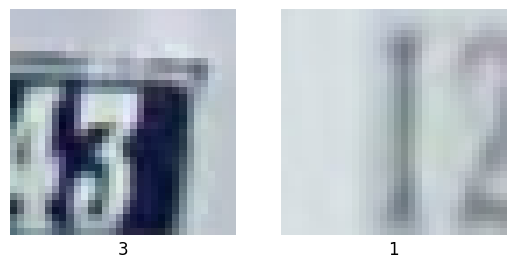
\includegraphics[width=\textwidth]{Bilder/svhn-examples.png}
		\caption{SVHN}
	\end{subfigure}
	\begin{subfigure}{0.32\textwidth}
		\centering
		
\includegraphics[width=\textwidth]{Bilder/mnist-examples.png}
		\caption{MNIST}
	\end{subfigure}
	\begin{subfigure}{0.32\textwidth}
		\centering
		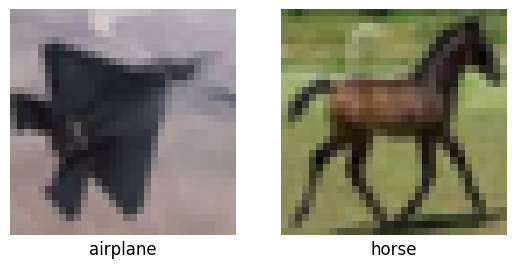
\includegraphics[width=\textwidth]{Bilder/cifar10-examples.png}
		\caption{CIFAR-10}
	\end{subfigure}
	\caption{Examples from the three training datasets}
	\label{fig:dataset-examples}
\end{figure}

\section{Environment}
Ich habe den Algorithmus aus \autoref{chap:methods} mit Python in Tensorflow Federated implementiert. Das ist ein auf Tensorflow aufgebautes Framework, das das Federated Training von Neuronalen Netzen, die in Tensorflow definiert werden, relativ einfach gestaltet. Das Framework ist sehr modular aufgebaut und erlaubt es Schritte im Federated Learning, wie zum Beispiel die Aggregation der Updates durch eine andere Aggregation auszutauschen. Abgesehen vom Federated Learning hat das Framework mit Federated Core den Anspruch, eine Basis für verteilte Berechnungen zu sein. Dafür hat es beispielsweise Datentypen so adaptiert, dass sie abgesehen vom eigentlichen Datentypen immer auch die Geräte beinhalten, an denen sie sich befinden. Die High-level Federated Learning API beinhaltet typische Algorithmen wie \texttt{FedAvg} oder \texttt{DP-FedAvg}.

\autoref{alg:boenisch-sample} habe ich so adaptiert, dass statt Opacus die Bibliothek \textit{dp-accounting} genutzt wird. Ich habe mich dazu entschieden, da der Rest meines Environments auf Tensorflow basiert und ich daher PyTorch nicht als weitere Abhängigkeit haben wollte.

Die Berechnungen habe ich auf dem Clara Cluster der Universität Leipzig ausgeführt. Um das Environment aufzusetzen und zu definieren habe ich ein Docker Image definiert, welches Python, CUDA und notwendige Bibliotheken installiert.

\section{Datasets}

\begin{figure}[tb]
	\centering
	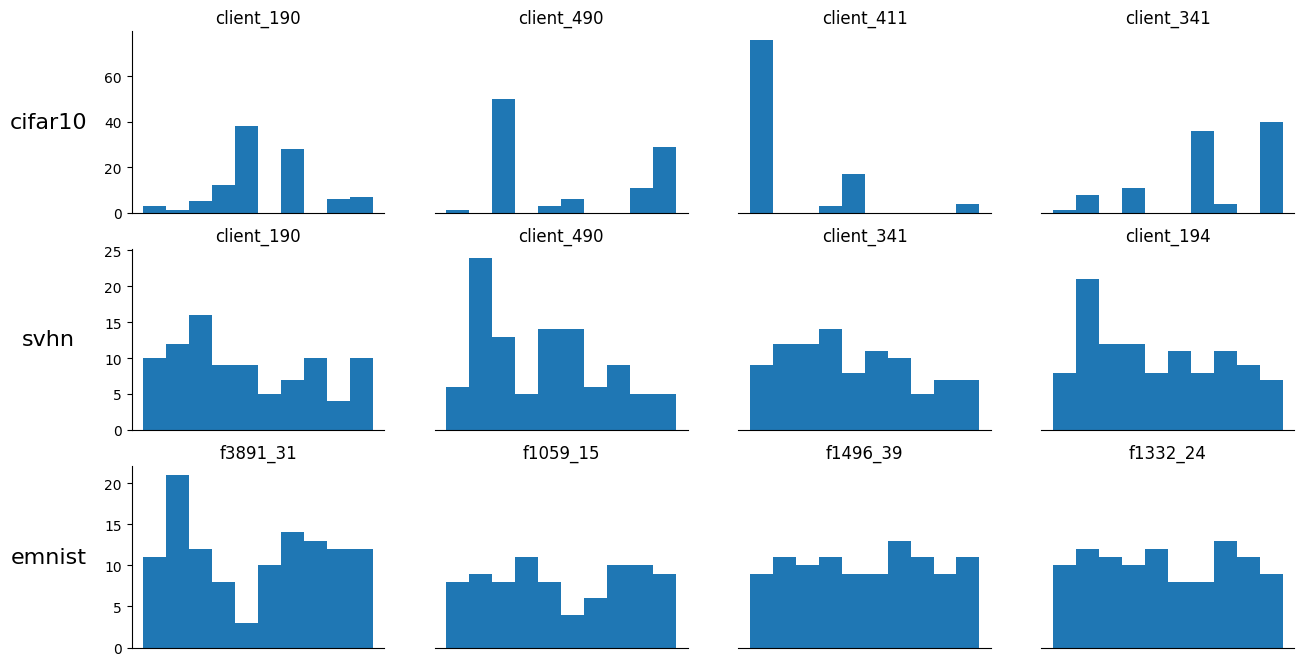
\includegraphics[width=\textwidth]{Bilder/label_distribution.png}
	\caption{Label distribution on exemplary clients from the different datasets}
	\label{fig:label-distribution}
\end{figure}

Der MNIST-Datensatz (Modified National Institute of Standards and Technology) ist ein weit verbreiteter Benchmark im Bereich des maschinellen Lernens, insbesondere für Bildklassifizierungsaufgaben. Er besteht aus 70.000 Graustufenbildern handgeschriebener Ziffern, wobei jedes Bild eine Größe von 28x28 Pixeln hat. Der Datensatz ist in 60.000 Trainingsbilder und 10.000 Testbilder unterteilt, wobei die Ziffern von 0 bis 9 reichen. Jedes Bild ist mit der entsprechenden Ziffer beschriftet, was es zu einem überwachten Lernproblem macht. Aufgrund seiner Einfachheit und Relevanz wird der MNIST-Datensatz häufig zum Testen neuer Algorithmen und Modelle in Aufgaben wie der Ziffernerkennung verwendet.

Tensorflow Federated stellt einen Datensatz bereit, der auf einer erweiterten Version von MNIST basiert. Die Ziffern sind dabei nach ihrem jeweiligen Autor aufgeteilt, was eine realistische Annahme im Federated Learning ist. Die Methodik bei der Aufteilung folgt \textcite{caldas:2018}. So wird ein \textit{Feature Distribution Skew} aus \autoref{fund-fl-data-heterogenity} simuliert. In \autoref{fig:emnist-feature-skew} ist die handgeschriebene Ziffer 8 von verschiedenen Clients zu sehen. Die unterschiedlichen Handschriften sind klar zu erkennen und stellen in diesem Datensatz die Verzerrung der Features dar.

\begin{figure}[tb]
	\centering
	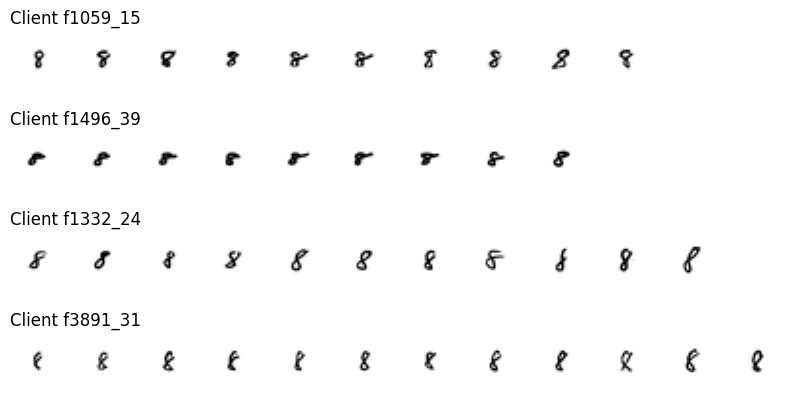
\includegraphics[width=0.8\textwidth]{Bilder/emnist_feature_distribution_skew.png}
	\caption{The digit eight from different clients in MNIST showing the different handwritings}
	\label{fig:emnist-feature-skew}
\end{figure}

\begin{figure}[tb]
	\centering
	\begin{subfigure}{0.32\textwidth}
		\centering
		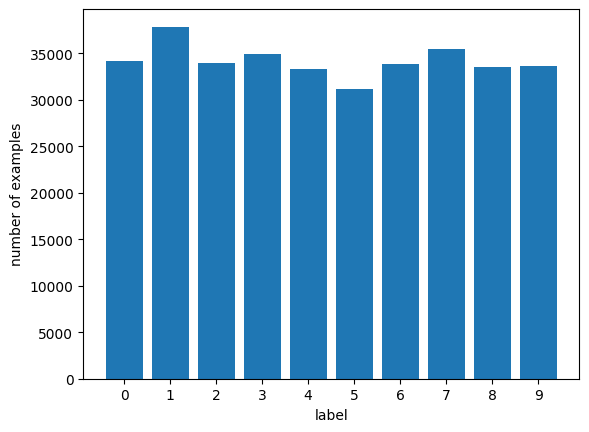
\includegraphics[width=\textwidth]{Bilder/emnist_label_distribution.png}
		\caption{MNIST}
	\end{subfigure}
	\begin{subfigure}{0.32\textwidth}
		\centering
		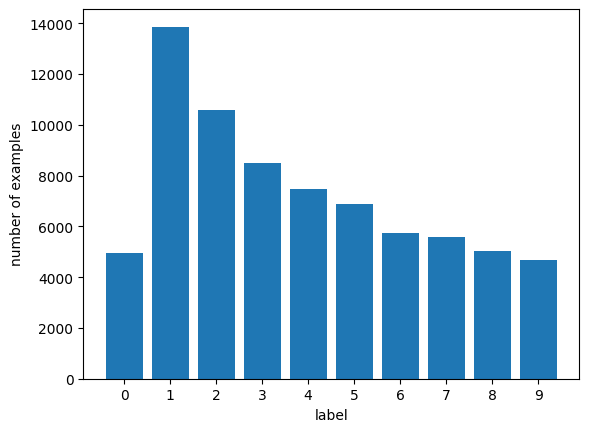
\includegraphics[width=\textwidth]{Bilder/svhn_label_distribution.png}
		\caption{SVHN}
	\end{subfigure}
	\begin{subfigure}{0.32\textwidth}
		\centering
		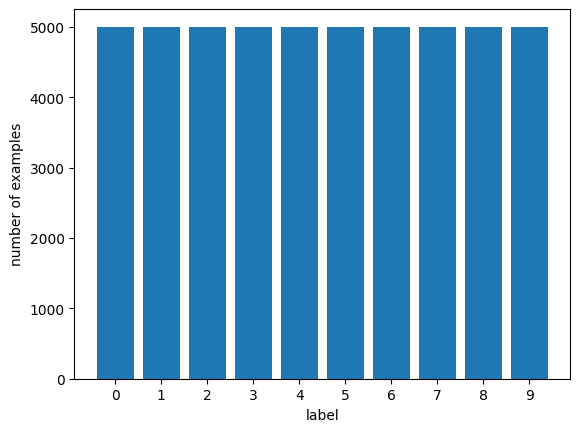
\includegraphics[width=\textwidth]{Bilder/cifar_label_distribution.png}
		\caption{CIFAR-10}
	\end{subfigure}
	\caption{Distribution of labels in the training datasets among all clients}
	\label{fig:label-distribution-all}
\end{figure}

Der SVHN-Datensatz (Street View House Numbers) ist ein weiterer bekannter Datensatz im Bereich des maschinellen Lernens, der häufig für Bildklassifizierungsaufgaben verwendet wird, speziell zur Erkennung von Ziffern. Er besteht aus über 600.000 farbigen Bildern von Hausnummern, die aus Google Street View-Aufnahmen extrahiert wurden. Jedes Bild enthält eine Ziffer (0-9) und ist in verschiedene Datensätze für Training und Testen unterteilt. Im Gegensatz zum MNIST-Datensatz, der handgeschriebene Ziffern zeigt, stellt SVHN ein anspruchsvolleres Problem dar, da die Ziffern aus der realen Welt stammen und häufig von komplexen Hintergründen, Beleuchtungsschwankungen und verschiedenen Schriftarten beeinflusst werden. SVHN ist daher ein wertvoller Datensatz zur Entwicklung und Evaluierung von Algorithmen, die unter realen Bedingungen gut funktionieren.

Es gibt keine Version dieses Datensatzes innerhalb von Tensorflow Federated, daher habe ich die Trainingsdaten zufällig auf eine Anzahl von Clients verteilt. Um zu verhindern, dass Clients jedes Mal andere Daten zugewiesen werden, habe ich den erstellten Datensatz in dem Tensorflow Federated \texttt{SqlClientData}-Format\footnote{\url{https://www.tensorflow.org/federated/api_docs/python/tff/simulation/datasets/SqlClientData} (accessed 28-11-2024)} gespeichert.

Der CIFAR-10-Datensatz (Canadian Institute For Advanced Research) ist ein bekannter Benchmark-Datensatz im Bereich des maschinellen Lernens und der Bildklassifikation. Er enthält 60.000 farbige Bilder mit einer Größe von 32x32 Pixeln, die in 10 verschiedene Klassen unterteilt sind: Flugzeuge, Autos, Vögel, Katzen, Hirsche, Hunde, Frösche, Pferde, Schiffe und Lastwagen. Jede Klasse ist mit 6.000 Bildern repräsentiert, und der Datensatz ist in 50.000 Trainingsbilder und 10.000 Testbilder aufgeteilt. CIFAR-10 stellt eine größere Herausforderung als einfachere Datensätze wie MNIST dar, da die Bilder vielfältigere und komplexere Objekte aus der realen Welt enthalten. 

Tensorflow Federated beinhaltet zwar keine Version des CIFAR-10 Datensatzes, allerdings gibt es den CIFAR-100-Datensatz \cite{krizhevsky:2009}. Jedoch ist dieser noch komplexer, daher habe ich mich entschlossen den CIFAR-10 Datensatz so aufzubereiten, wie es beim Tensorflow Federated CIFAR-100 Datensatz gemacht wurde. 

Dort wird für jeden Client ein Vektor aus der Dirichlet-Verteilung gezogen, welcher für jede Klasse die Wahrscheinlichkeit repräsentiert, ein Trainingsbeispiel aus der jeweiligen Klasse zu ziehen. Dementsprechend zieht jeder Client Beispiele aus dem Datensatz. Wenn eine Klasse keine weiteren Daten enthält, wird der Zahlenvektor für jeden Client neu gezogen, allerdings nur mit den Klassen, die noch nicht aufgebraucht sind. Am Ende erhält man so Clients, bei denen die Klassen je nach Client unterschiedlich stark vertreten sind und es wird ein \textit{Label Distribution Skew} aus \autoref{fund-fl-data-heterogenity} abgebildet. Der Effekt ist in \autoref{fig:label-distribution} zu sehen. Die Verteilung der Klassen bei den CIFAR-10 Clients ist sehr viel unregelmäßiger als die der anderen Datensätze und hat viele Lücken.

\autoref{fig:label-distribution-all} zeigt die Verteilung der Labels in den gesamten Trainingsdaten. Es ist auffällig, dass es in SVHN deutlich mehr kleinere Ziffern gibt als größere, mit Ausnahme der $0$. Allerdings lässt sich das womöglich dadurch erklären, dass Hausnummern in der Regel aufsteigend vorliegen und es daher für jede Ziffer $9$ auch $1$ bis $8$ gegeben haben muss. Diese ungleiche Verteilung wirkt sich, wie in \autoref{fig:label-distribution} zu sehen ist, auch auf die Menge der Trainingsbeispiele auf den Clients aus.

\section{Exemplary setup of individual sampling rates and the noise multiplier}
Um zu veranschaulichen, wie welche Trainingsparameter zu welchen Sampling Rates für den Algorithmus führen und die Auswirkungen zu zeigen, habe ich diese für leicht variierte Setups berechnet. Ich zeige dies ausgehend von den Parametern des MNIST-Datensatzes. Dieser umfasst $3383$ Clients, dementsprechend wähle ich $\delta= 1e-5$. 

Zunächst verteile ich die Privacy Budgets mit der Verteilung $[0.34, 0.43, 0.23]$ unter den Clients. Die konkrete Zuweisung der Budgets anhand dieser Verteilung unterliegt dem Zufall, kann also leicht variieren. Mit Privacy-Budgets von $\epsilon = [1,2,3]$, $50$ Clients pro Runde und 100 Runden berechnet \autoref{alg:boenisch-sample} einen Noise Multiplier $\sigma = 0.92$ und Sampling Rates für die Budgets von $q = [0.003, 0.016, 0.028]$. Wie gefordert liegt der Erwartungswert der Clients pro Runde ungefähr bei $50$, genau bei $50.078$.

Wenn die Budgets auf $\epsilon = [10, 20, 30]$ erhöht werden, ändern sich die Sampling Rates leicht, vor allem sinkt aber der Noise Multiplier auf $\sigma = 0.38$. Das führt dazu, dass im weiteren Training die Gradienten deutlich weniger verrauscht werden.

Bei einer Verteilung der Budgets unter den Clients, die mehr Clients mit strengeren Budgets erzeugt, steigt $\sigma$ ebenfalls. Auch die Sampling Rates ändern sich deutlich. Bei einer Verteilung von $[0.54, 0.37, 0.09]$ steigt der Noise Multiplier auf $\sigma = 0.99$ und die Sampling Rates liegen bei $q = [0.006, 0.022, 0.036]$. Das führt auf der neuen Verteilung zu $50.072$ erwarteten Clients pro Runde.

Wenn die Clients pro Runde gleich bleiben, aber die Anzahl der Clients im Datensatz herabgesetzt wird, steigt der Noise Multiplier ebenfalls. Das liegt daran, dass ein einzelner Client damit im Training häufiger gezogen wird und deshalb sein Beitrag zu dem Modell wieder stärker begrenzt werden muss um seine Privatheit zu schützen. Die Sampling Rates verändern sich auch, allerdings bleibt die Anzahl der Clients pro Runde im Mittel erhalten. Wenn statt den $3383$ Clients nur $1000$ Clients angenommen werden steigt der Noise Multiplier auf $\sigma = 1.50$. In der Praxis würde das natürlich auch dazu führen, dass es pro Client mehr Daten geben würde, also die Updates zwar stärker verrauscht werden würden, aber vermutlich auch aussagekräftiger wären.

Ähnlich ist es, wenn die Anzahl der Trainingsrunden erhöht wird. Auch hier wird ein einzelner Client innerhalb des Trainings vermutlich häufiger gezogen, als bei weniger Runden. Bei $1000$ Runden steigt der Noise Multiplier auf $\sigma = 1.32$

Auch wenn die Clients pro Runde erhöht werden ist das der Fall. Bei $200$ statt den bisherigen $50$ Clients pro Runde liegt der Noise Multiplier bei $\sigma = 1.68$.



\section{IID versions of the datasets}\label{sec:iid-dataset-creation}
Für MNIST und CIFAR-10 erstelle ich abgesehen von den oben genannten Datensätzen noch eine Version, bei der die Daten zufällig auf den Clients verteilt werden. Der Grund dafür ist, dass \texttt{FedAvg}, auf dem mein Algorithmus basiert, Schwierigkeiten mit Verzerrungen in den Trainingsdaten hat. Diese Versionen sollen also vor allem als eine Baseline sein und zur Vergleichbarkeit meiner Ergebnissen beitragen.

\textit{Tensorflow Federated} stellt für die Erstellung gleichverteilter Datensätze eine Funktion bereit.\footnote{\url{https://www.tensorflow.org/federated/api_docs/python/tff/simulation/datasets/build_synthethic_iid_datasets}, (accessed 07-11-2024)} Diese erstellt einen \texttt{Iterator}, bei dem in jeder Iteration zufällig aus allen Trainingsdaten gezogen wird. Damit gibt es jedoch keine Zuweisung mehr von den Daten zu den Clients, das heißt wenn ein Client gezogen wird, werden seine Trainingsdaten dynamisch zusammengesetzt.

Ich wollte in meinem Fall gerne eine Beziehung der Clients zu den Daten beibehalten, das heißt wenn in meinem Fall der gleiche Client in verschiedenen Runden gezogen wird, trainiert er auch auf den gleichen Daten.

Dazu habe ich eine Funktion geschrieben, die einen Datensatz als Eingabe bekommt und dann die Datenpunkte zufällig den Clients zuweist. Diese Funktion liefert dann einen Datensatz zurück in dem Clients feste Datenpunkte zugewiesen sind.

\section{Model Architecture}
Die Datensätze, auf denen ich meinen Algorithmus auswerte sind für Bildklassifizierungen gemacht. Daher verwende ich in meinen Experimenten ein einfaches Convolutional Neural Network. Das Neuronale Netz ist für alle Datensätze das gleiche, lediglich die \texttt{input\_shape} passe ich den jeweiligen Daten an. Außerdem gibt es einen Rescaling Layer, der die Pixel auf das Intervall $[0;1]$ normalisiert. Bei MNIST ist das nicht nötig, da bereits alle Werte zwischen $0$ und $1$ liegen.

Das Neuronale Netz selbst ist sehr klein und enthält nur $21578$ trainierbare Parameter. Ich habe mich dafür entschieden, das Training damit durchzuführen, da größere Modelle einen erheblichen Mehraufwand beim Training bedeuten, weil im Trainingsprozess viele Clients simuliert werden müssen. Bereits bei auf Effizienz ausgerichteten Modellen wie \textit{MobileNet} \cite{howard:2017} und \textit{EfficientNet} \cite{tan:2019} war ein zügiges Training nicht mehr möglich.

Die Schichten des Modells bestehen aus Convolutional, MaxPooling und Dropout Layern. Darüber hinaus gibt es am Ende zwei Linear Layers für die Klassifikation.

\begin{figure}[tb]
	\centering
	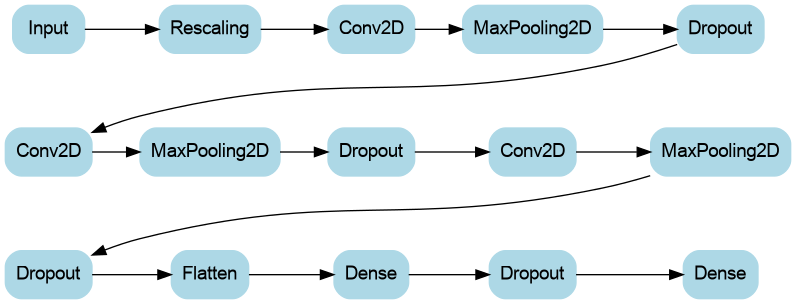
\includegraphics[width=0.8\textwidth]{Bilder/model_architecture_1.png}
	\caption{Architecture of the model used for the classification tasks}
	\label{fig:model-architecture}
\end{figure}

Um das Training einfach zu halten habe ich auf weitere Vorverarbeitungsschritte der Bilder verzichtet. Ich führe auch keine Augmentation der Trainingsdaten durch, zum Beispiel durch zufälliges drehen oder zuschneiden der Bilder.

Durch lokale Experimente auf zentralen Trainingsdaten habe ich überprüft, dass mein Modell auf allen Datensätzen in der Lage ist zu lernen. Daher ist das Modell für mein Ziel ausreichend, nämlich meinen Trainingsalgorithmus zu testen und Aussagen über die Auswirkungen verschiedener Parameter zu treffen.

\section{Privacy Setups}
Ich führe die Experimente jeweils mit insgesamt fünf Privacy-Niveaus durch. Im folgenden werde ich mich mit den Namen \texttt{no-dp}, \texttt{relaxed-dp}, \texttt{relaxed-idp}, \texttt{strict-idp} und \texttt{strict-dp} auf diese beziehen. In dieser Reihenfolge haben sie ansteigende Anforderungen an die Differential Privacy. \autoref{tab:privacy-niveau-distribution} zeigt die Verteilung der Privacy Budgets für jedes der Setups. \texttt{strict-idp} und \texttt{relaxed-idp} sind die beiden Setups, die mit individualisierten Privacy Budgets arbeiten. Die anderen nutzen entweder homogene Budgets oder gar keine und dienen zum Vergleich mit meinen Ergebnissen. Die Erwartung ist, dass \texttt{no-dp} und \texttt{relaxed-dp} besser abschneiden, als \texttt{relaxed-idp} und \texttt{strict-idp}, während \texttt{strict-dp} die größten Abstriche bei der Nützlichkeit erwarten lässt.

\begin{table}[tb]
	\centering
	\begin{tabular}{|c|c|c|c|}
		\hline
		Level & $\epsilon_1$ & $\epsilon_2$ & $\epsilon_3$ \\
		\hline
		\texttt{no-dp} & - & - & - \\
		\texttt{relaxed-dp} & - & - & $100\%$ \\
		\texttt{relaxed-idp} & $34\%$ & $43\%$ & $23\%$ \\
		\texttt{strict-idp} & $54\%$ & $37\%$ & $9\%$ \\
		\texttt{strict-dp} & $100\%$ & - & - \\
		\hline
	\end{tabular}
	\caption{The distribution of Privacy Budgets in the different Privacy Setups with $\epsilon_1$ being the smallest, $\epsilon_2$ the intermediate and $\epsilon_3$ the largest Privacy Budget}
	\label{tab:privacy-niveau-distribution}
\end{table}

Für jeden Datensatz definiere ich drei Privacy-Budgets jeweils für Clients die niedrige, mittlere und hohe Anforderungen an ihre Privatheit haben. Ich musste in meinen Experimenten feststellen, dass einheitliche Budgets über alle Datensätze nicht funktionieren, weil die Modelle dann bei SVHN und CIFAR-10 nicht konvergieren. Das unterstreicht noch einmal unterschiedlichen Schwierigkeitsgrade zwischen den Datensätzen und deckt sich tendenziell mit den Erfahrungen von \textcite{sun:2021}.

\begin{table}[tb]
	\centering
	\begin{tabular}{|c|c|c|c|}
		\hline
		Dataset & $\epsilon_1$ & $\epsilon_2$ & $\epsilon_3$ \\
		\hline
		MNIST & $1.0$ & $2.0$ & $3.0$ \\
		SVHN & $15.0$ & $25.0$ & $40.0$ \\
		CIFAR10 & $15.0$ & $25.0$ & $40.0$ \\
		\hline
	\end{tabular}
	\caption{The Privacy Budgets for each dataset}
	\label{tab:privacy-budgets-per-dataset}
\end{table}

Die Annahmen, dass es drei Gruppen mit unterschiedlichen Anforderungen an die Privatheit gibt und auch die Verteilungen dieser Gruppen innerhalb der Clients folgt \textcite{boenisch:2023} und ist durch empirische Studien gedeckt \cite{jensen:2005, acquisti:2005}. Eine Übersicht der Budgets auf den Datensätzen steht in \autoref{tab:privacy-budgets-per-dataset}.

%\begin{table}[tb]
%	\centering
%	\begin{tabular}{|c|c|c|c|c|c|c|c|}
%		\hline
%		\multirow{2}{4em}{Dataset} & \multicolumn{3}{|c|}{Whole Dataset} & \multicolumn{4}{|c|}{Per Client} \\
%		\cline{2-8}
%		& \#examples & \#classes & \#clients & $\diameter$examples & $\sigma$examples & $\diameter$classes & $\sigma$classes \\
%		\hline
%		MNIST & 341873 & 10 & 3383 & 101.05 & 14.72 & 9.99 & 0.14 \\
%		SVHN & 26032 & 10 & 725 & 35.91 & 5.89 & 9.45 & 0.76 \\
%		CIFAR-100 & 50000 & 20 & 500 & 100.0 & 0.0 & 6.53 & 1.99 \\
%		\hline
%	\end{tabular}
%	\caption{Some statistics of the different datasets for (1) the whole dataset and (2) the individual clients}
%	\label{tab:dataset-statistics}
%\end{table}



\chapter{Ergebnisse}\label{chap:results}
%\begin{itemize}
%	\item Hyperparameter beschreiben (Clients pro Runde, Learning Rate yadayadayada)
%	\item Numerisch beschreiben was es für Unterschiede gibt (bei iid ist das Delta von der Privacy setups so und so usw)
%	\item $\delta$'s pro Datensatz erwähnen und sagen wie ich sie gewählt habe
%\end{itemize}

In diesem Kapitel gehe ich auf die Ergebnisse der Experimente aus \autoref{chap:experiments} ein. In \autoref{sec:non-fl-training-results} beschreibe ich Ergebnisse von lokalen Trainingsdurchläufen mit dem identischen Modell. In \autoref{sec:fl-training-results} erläutere ich detaillierter, welche Ergebnisse ich im Federated Learning erzielt habe und beschreibe die genutzten Hyperparameter.

\section{Non-federated Training} \label{sec:non-fl-training-results}
Die Ergebnisse der lokalen Trainingsdurchläufe sind, wie zu erwarten, etwas besser als im Federated Learning, auch wenn sie nicht der \textit{state-of-the-art} entsprechen. Das liegt an dem einfachen und kleinen Modell, das ich für das Training genutzt habe.

Bei MNIST und SVHN erreicht das Modell bereits innerhalb von 10 Epochen gute Ergebnisse. Bei CIFAR-10 sind die Ergebnisse deutlich schlechter, weshalb ich hier mit einem \texttt{EarlyStopping}-Callback gearbeitet habe, der abbricht sobald das Modell \textit{overfittet}. Trotzdem liegt die erreichte Accuracy unter 50\%. Eine Übersicht zeigt \autoref{tab:local-model-results}.

\begin{table}
	\centering
	\begin{tabular}{ccc}
		\toprule
		Dataset & Accuracy & Loss \\
		\midrule
		MNIST & 0.9842 & 0.0535 \\
		SVHN & 0.8758 & 0.4203 \\
		CIFAR-10 & 0.634 & 1.0395 \\
		\bottomrule
	\end{tabular}
	\caption{Die Ergebnisse von nicht privaten und zentral durchgeführten Trainingsdurchläufen}
	\label{tab:local-model-results}
\end{table}

Allerdings liegt der Fokus meiner Arbeit auf dem Federated Learning Algorithmus und die lokalen Trainingsdurchläufe sollten vor allem zum Vergleich und zum Finden von angemessenen Modellen und Hyperparametern dienen. Sie waren hilfreich, denn ich konnte beispielsweise mein Convolutional Neural Network mit einem Feed-Forward Netz vergleichen. 

Die Trainingszeit liegt bei wenigen Sekunden oder Minuten. Derartige Experimente wären im Federated Learning sehr viel umständlicher gewesen, da das Training einen deutlich erhöhten Rechenaufwand mit sich bringt und auch, was die Konvergenz der Modelle betrifft, instabiler ist.

\begin{figure}
	\centering
	\begin{subfigure}{0.32\textwidth}
		\centering
		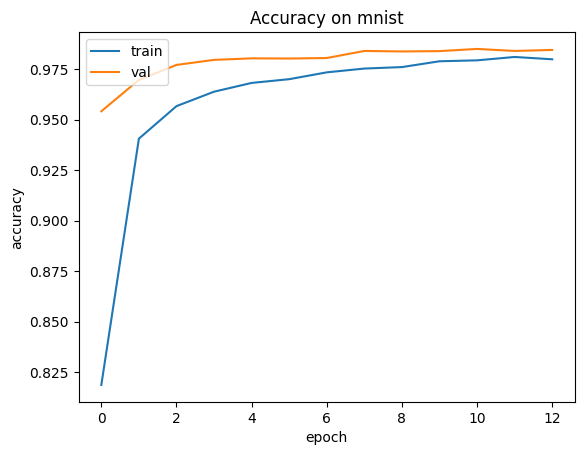
\includegraphics[width=\textwidth]{Bilder/mnist-results-local.png}
		\caption{MNIST}
	\end{subfigure}
	\begin{subfigure}{0.32\textwidth}
		\centering
		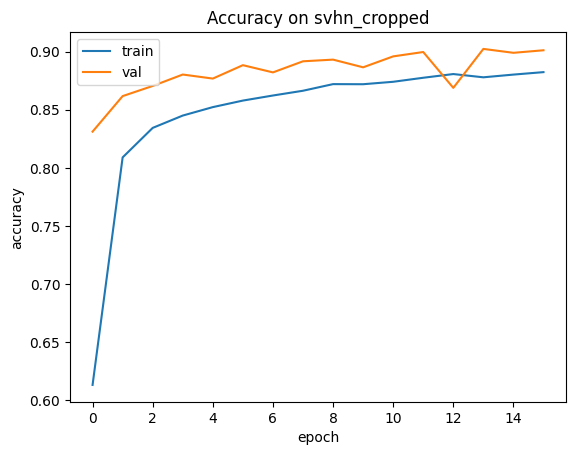
\includegraphics[width=\textwidth]{Bilder/svhn-results-local.png}
		\caption{SVHN}
	\end{subfigure}
	\begin{subfigure}{0.32\textwidth}
		\centering
		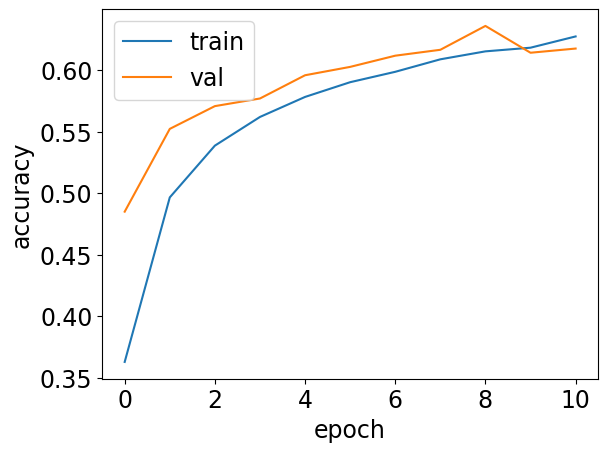
\includegraphics[width=\textwidth]{Bilder/cifar-results-local.png}
		\caption{CIFAR-10}
	\end{subfigure}
	\caption{Genauigkeiten auf den Trainings- und Validierungsdatensätzen im nicht-privaten, zentralen Training}
	\label{fig:local-training-histories}
\end{figure}

\section{Federated Training}\label{sec:fl-training-results}

Die Ergebnisse des Trainings im Federated Learning sind in \autoref{tab:all-fed-results} zu sehen. Die Ergebnisse sind nach den Datensätzen aufgeteilt und jeweils für die normale Version (\textit{non-i.i.d.}) und die unabhängig gleichverteilte Version (\textit{i.i.d.}) notiert. Die gleichverteilte Version ist durch das in \autoref{sec:iid-dataset-creation} beschriebene Verfahren entstanden.

Die Genauigkeit bezieht sich in jedem Fall auf die Auswertung des Modells auf den Testdaten. Für die Evaluierung habe ich die Testdaten zu einem zentralen Datensatz zusammengefügt und dann das Modell darauf evaluiert. Eine andere Möglichkeit wäre gewesen, die Evaluierung ebenfalls auf den Clients durchzuführen. Für den Fall, dass man ein vortrainiertes Modell für jeden Client noch einmal nachtrainiert, damit es auf seinen Daten gut funktioniert, wäre diese Art der Evaluierung angemessener gewesen. Allerdings war ich nur an der allgemeinen Performanz des Modells interessiert.

Es ist auffällig, dass die Modelle auf allen Datensätzen in der gleichverteilten Version besser abschneiden. Das deckt sich mit dem Stand der Forschung zu \texttt{FedAvg}.

\begin{table}
	\centering
	\begin{tabular}{lp{4em}p{4em}p{4em}p{4em}p{4em}p{4em}}
		\toprule 
	 	& \multicolumn{2}{c}{MNIST} & \multicolumn{2}{c}{SVHN} & \multicolumn{2}{c}{CIFAR-10} \\
		\cmidrule(lr){2-3}\cmidrule(lr){4-5}\cmidrule(lr){6-7}
		& i.i.d. & non-i.i.d. & i.i.d. & non-i.i.d. & i.i.d. & non-i.i.d. \\
		\midrule
		\texttt{no-dp} & 0.906 & 0.896 & 0.825 & - & 0.419 & 0.246 \\
		\texttt{relaxed-dp} & 0.931 & 0.855 & 0.544 & - & 0.407 & 0.252 \\
		\texttt{relaxed-idp} & 0.917 & 0.883 & 0.418 & - & 0.394 & 0.255 \\
		\texttt{strict-idp} & 0.91 & 0.887 & 0.446 & - & 0.386 & 0.235 \\
		\texttt{strict-dp} & 0.895 & 0.811 & 0.292 & - & 0.387 & 0.246 \\
		\bottomrule
	\end{tabular}
	\caption{Mit den verschieden Privacy Setups erzielte Genauigkeiten im Federated Training}
	\label{tab:all-fed-results}
\end{table}

\subsection{Hyperparameter Setups}
Ich habe das Training mit allen Datensätzen auf $100$ Runden begrenzt. Grund dafür war einerseits die Trainingszeiten kurz zu halten, andererseits gibt es auch eine Wechselwirkung mit der Anzahl der Runden und dem Privacy Loss. Bei einer höheren Rundenzahl erhöht er sich, denn jeder Client wird im Verlauf des Trainings häufiger oder mit einer größeren Wahrscheinlichkeit gezogen. Daher muss im Umkehrschluss das Rauschen größer werden. 

Ein weiterer Hyperparameter, der einen Einfluss auf die Stärke des Rauschens hat, ist die Anzahl der Clients, die pro Runde gezogen werden sollen. Davon hängt die Wahrscheinlichkeit mit der die Clients gezogen werden ab. Hier gilt ebenso, dass bei einer größeren Wahrscheinlichkeit die Daten eines Clients einen größeren Einfluss auf das trainierte Modell haben und damit das Rauschen vergrößert werden muss.

Hyperparameter, die sich nicht auf den Privacy Loss auswirken sind die Learning Rates auf dem Server und die Learning Rates auf den Clients. Auch die Anzahl der Epochen, die jeder Client auf seinen Daten trainiert, und die Größe der Batches wirken sich nicht auf den Privacy Loss aus.

Wie in \autoref{chap:methods} beschrieben, verwende ich für die Hyperparameter des \textit{Adaptive Clippings} die Standardwerte.

\begin{table}[tb]
	\centering
	\begin{tabular}{lccc}
		\toprule
		Hyperparameter & MNIST & SVHN & CIFAR-10 \\
		\midrule
		Rounds & 100 & 100 & 100 \\
		Clients per round & 50 & 30 & 30 \\
		Batchsize & 128 & 128 & 128 \\
		Local Epochs & 5 & 5 & 5 \\
		Client learning rate & 0.001 & 0.001 & 0.001 \\
		Server learning rate & 1.0 & 1.0 & 1.0 \\
		\bottomrule
	\end{tabular}
	\caption{Hyperparameter, die auf den verschiedenen Datensätzen genutzt wurden}
	\label{tab:fl-hyperparameters}
\end{table}

\subsection{MNIST}

Bei MNIST konnten die DP-Algorithmen ähnlich gute Ergebnisse erzielen wie das nicht-private \texttt{FedAvg}. In \autoref{fig:fed-emnist-results} ist dennoch ein Einfluss des Privacy Setups auf das Ergebnis zu sehen. Vor allem \texttt{strict-dp} konvergiert ein bisschen instabiler und kommt nicht ganz an die anderen Ergebnisse heran. Außerdem fällt der Loss bei \texttt{no-dp} bereits deutlich früher ab. Bei den anderen Setups erfolgt die Absenkung erst nach ungefähr 15 Runden. Die restlichen Privacy-Niveaus liegen sehr nah beieinander, allerdings ist auffällig, dass \texttt{relaxed-dp} schlechter abschneidet, als die individualisierten Niveaus.

\begin{figure}[h]
	\centering
	\begin{subfigure}{0.45\textwidth}
		\centering
		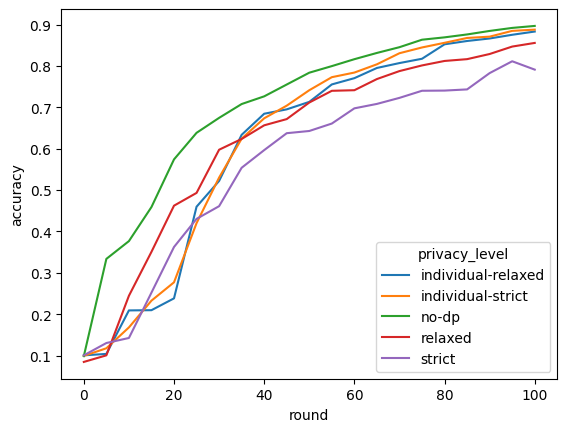
\includegraphics[width=\textwidth]{Bilder/emnist-accuracy.png}
		\caption{Genauigkeit auf Validierungsdaten (non-i.i.d)}
	\end{subfigure}
	\begin{subfigure}{0.45\textwidth}
		\centering
		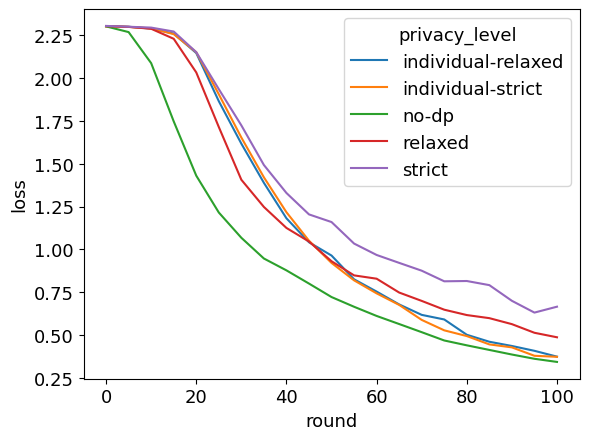
\includegraphics[width=\textwidth]{Bilder/emnist-loss.png}
		\caption{Loss auf Validierungsdaten (non-i.i.d)}
	\end{subfigure}
	\begin{subfigure}{0.45\textwidth}
		\centering
		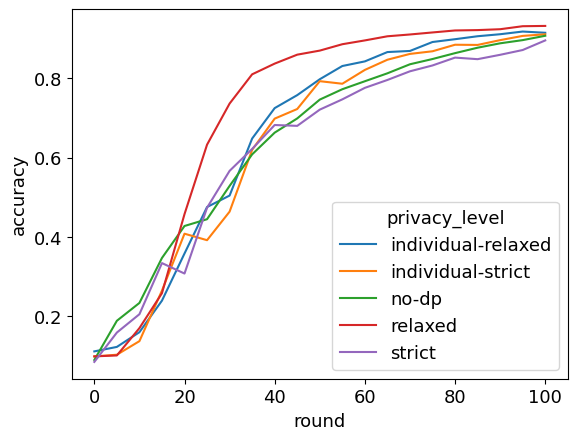
\includegraphics[width=\textwidth]{Bilder/emnist-accuracy-iid.png}
		\caption{Genauigkeit auf Validierungsdaten (i.i.d)}
	\end{subfigure}
	\begin{subfigure}{0.45\textwidth}
		\centering
		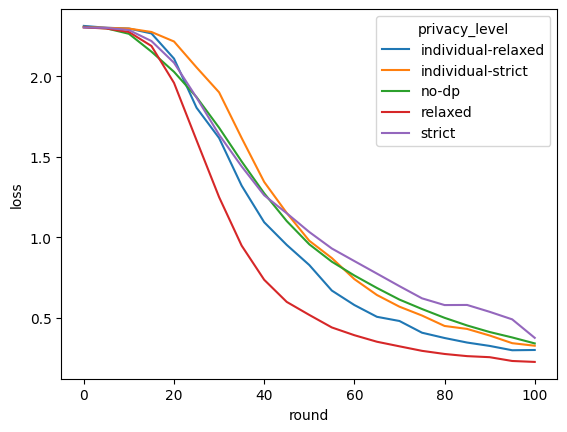
\includegraphics[width=\textwidth]{Bilder/emnist-loss-iid.png}
		\caption{Loss auf Validierungsdaten (i.i.d)}
	\end{subfigure}
	\caption{Genauigkeit und Loss der verschiedenen Privacy Setups im Verlauf des Trainings auf MNIST}
	\label{fig:fed-emnist-results}
\end{figure}

Die vorher berechneten Noise Multiplier für jedes Setup sind in \autoref{tab:noise-multipliers} zu sehen. Wie erwartet sind sie aufsteigend, je nach Größe des Privacy Budgets der Clients.

\begin{table}
	\centering
	\begin{tabular}{lccc}
		\toprule
		Setup & MNIST & SVHN & CIFAR-10 \\
		\midrule
		\texttt{no-dp} & - & - & - \\
		\texttt{relaxed-dp} & 0.769 & 0.348 & 0.384 \\
		\texttt{relaxed-idp} & 0.917 & 0.415 & 0.461 \\
		\texttt{strict-idp} & 1.000 & 0.444 & 0.494 \\
		\texttt{strict-dp} & 1.180 & 0.508 & 0.568 \\
		\bottomrule
	\end{tabular}
	\caption{Noise Multiplier der verschiedenen Setups}
	\label{tab:noise-multipliers}
\end{table}

Bei dem Training auf MNIST konnte ich mit $50$ Clients pro Runde im Erwartungswert gute Ergebnisse erzielen. Zwar würde man erwarten, dass das Modell mit mehr Clients in jeder Runde eine repräsentativere Stichprobe der Daten sieht, allerdings ist die Anzahl der Clients wie beschrieben ein Parameter der auch das Rauschen verstärkt. Daher konnte ich mit größeren Zahlen keine besseren Ergebnisse beobachten.

\subsection{SVHN}

Bei SVHN ist der Unterschied zwischen dem Training mit und ohne Differential Privacy sehr viel deutlicher zu sehen. Während die Metriken sich ohne Differential Privacy im Trainingsprozess kontinuierlich verbessern, hat jedes Setup mit Differential Privacy ab einem bestimmten Punkt im Training Probleme sich weiter zu verbessern. Vor allem \texttt{strict-dp} kann sich nur für kurze Zeit am Anfang verbessern. Bereits \texttt{relaxed-dp} erreicht kaum mehr eine halb so gute Genauigkeit wie das \texttt{no-dp}. Die beiden individualisierten Setups liegen noch ein wenig darunter, liefern allerdings deutlich bessere Ergebnisse als \texttt{strict-dp}. Auffällig ist, dass \texttt{strict-idp} noch ein bisschen besser abschneidet, als \texttt{relaxed-idp}, allerdings kann das Zufall sein.

Die Nähe der individualisierten Niveaus zu \texttt{relaxed-dp} und der Abstand zu \texttt{strict-dp} zeigt hier sehr deutlich den Vorteil der individualisierten Budgets. Während \texttt{relaxed-dp} zwar noch bessere Ergebnisse erzielt, werden hier die Abstriche bei der Privacy der Clients mit den Budgets $\epsilon_1$ bzw. $\epsilon_2$ sehr groß. Andererseits hält \texttt{strict-dp} zwar alle Budgets ein, da auf alle Clients $\epsilon_1$ angewendet wird, allerdings ist hier die Nützlichkeit des Modells stark beeinträchtigt.

Die \textit{Noise Multiplier} sind ebenfalls aufsteigend, allerdings sind sie insgesamt deutlich niedriger als bei MNIST. Dies zeigt, dass dieser Datensatz deutlich anfälliger gegenüber dem Hinzufügen von Rauschen ist und sich die Ergebnisse sehr schnell verschlechtern können.

\begin{figure}
	\centering
	\begin{subfigure}{0.45\textwidth}
		\centering
		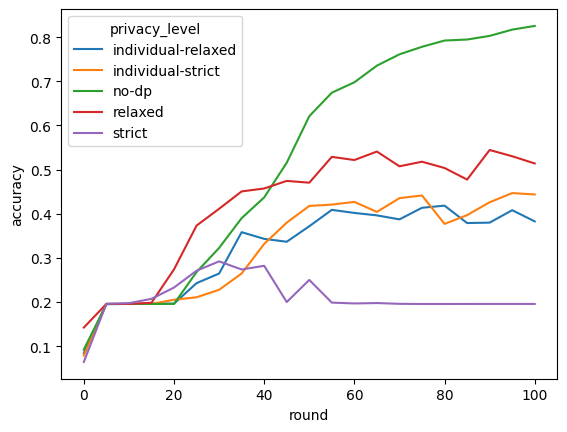
\includegraphics[width=\textwidth]{Bilder/svhn-accuracy.png}
		\caption{Genauigkeit auf Validierungsdaten}
	\end{subfigure}
	\begin{subfigure}{0.45\textwidth}
		\centering
		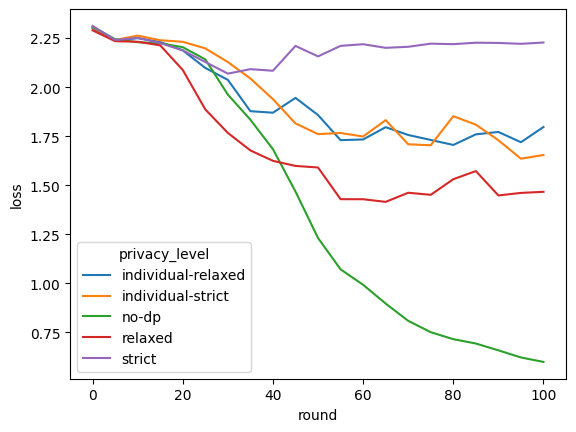
\includegraphics[width=\textwidth]{Bilder/svhn-loss.png}
		\caption{Loss auf Validierungsdaten}
	\end{subfigure}
	\caption{Genauigkeit und Loss der verschiedenen Privacy Setups im Verlauf des Trainings auf SVHN}
	\label{fig:fed-svhn-results}
\end{figure}

\subsection{CIFAR-10}
Bei CIFAR-10 ist auffällig, dass die Performanz des Modells kaum vom Privacy-Niveau abhängt, sondern eher von der Verteilung der Daten. Bei der ungleichmäßigen Verteilung mit dem \textit{Label Distribution Skew} verbessern sich alle Modelle nur sehr langsam und unstetig. Die Unterschiede zwischen den Privacy Niveaus selbst sind kaum zu erkennen.

Bei dem Training auf dem gleichverteilten Datensatz werden alle Modelle deutlich besser. Auch hier liegen die verschiedenen Privacy-Setups nah an dem nicht-privat trainierten Modell. Es fällt aber auf, dass die Verbesserungen der privat trainierten Modelle etwas weniger gleichmäßig ist. Zwischen den individualisierten und den homogenen Budgets ist kein großer Unterschied zu erkennen.

\begin{figure}[tb]
	\centering
	\begin{subfigure}{0.45\textwidth}
		\centering
		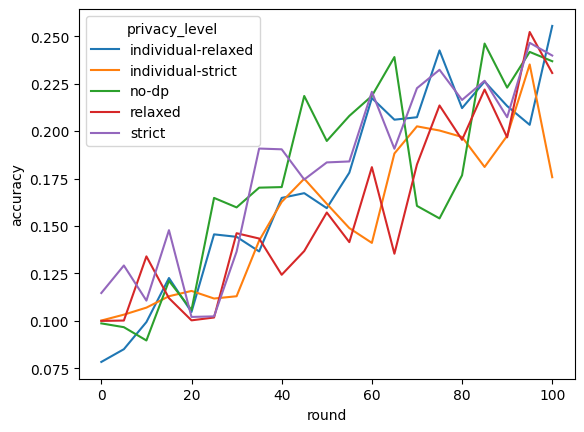
\includegraphics[width=\textwidth]{Bilder/cifar10-accuracy.png}
		\caption{Genauigkeit auf Validierungsdaten (non-i.i.d)}
	\end{subfigure}
	\begin{subfigure}{0.45\textwidth}
		\centering
		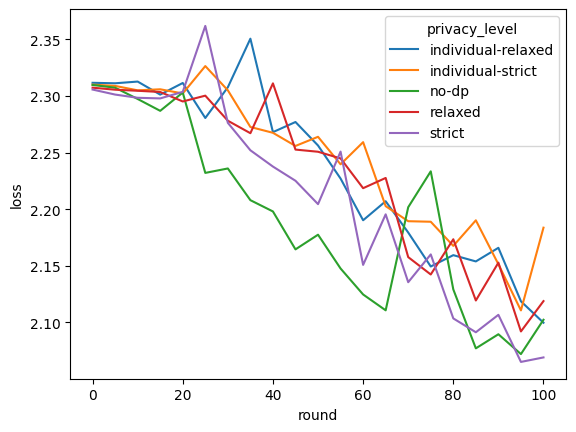
\includegraphics[width=\textwidth]{Bilder/cifar10-loss.png}
		\caption{Loss auf Validierungsdaten (non-i.i.d)}
	\end{subfigure}
	\begin{subfigure}{0.45\textwidth}
		\centering
		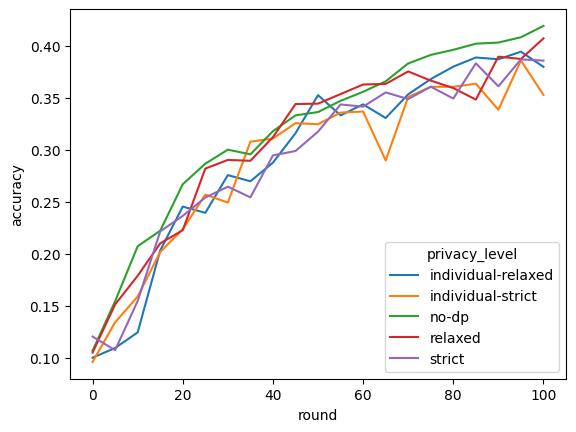
\includegraphics[width=\textwidth]{Bilder/cifar10-accuracy-iid.png}
		\caption{Genauigkeit auf Validierungsdaten (i.i.d)}
	\end{subfigure}
	\begin{subfigure}{0.45\textwidth}
		\centering
		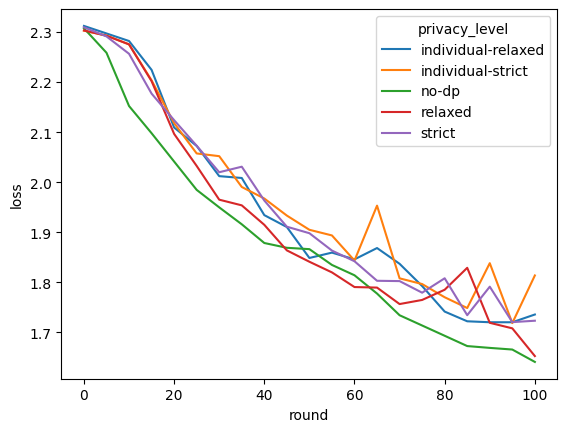
\includegraphics[width=\textwidth]{Bilder/cifar10-loss-iid.png}
		\caption{Loss auf Validierungsdaten (i.i.d)}
	\end{subfigure}
	\caption{Genauigkeit und Loss der verschiedenen Privacy Setups im Verlauf des Trainings auf CIFAR-10}
	\label{fig:fed-cifar10-results}
\end{figure}

\subsection{SVHN und CIFAR-10 mit kleineren Privacy Budgets}

Wie bereits erwähnt habe ich für CIFAR-10 und SVHN deutlich größere Privacy Budgets genutzt als für MNIST. Dies habe ich nicht willkürlich so festgelegt, sondern ich habe nach und nach größere Budgets ausprobiert. In \autoref{fig:cifar-svhn-small-budgets} sind die Trainingsverläufe mit kleineren Privacy Budgets zu sehen.

In der ersten Spalte sind die Trainingsverläufe mit den zu MNIST identischen Budgets von $\epsilon = \{1,2,3\}$ zu sehen. Bei CIFAR-10 fällt auf, dass bei \texttt{strict-dp} keine Verbesserung im Trainingsverlauf stattfindet. Die mit den individualisierten Niveaus trainierten Modelle können sich zunächst etwas verbessern, allerdings sinkt die Validation Accuracy im Verlauf des Trainings wieder.

Auf dem SVHN Datensatz verbessert sich keines der Modelle, die mit Differential Privacy trainiert werden. Alle bleiben beinahe konstant bei einer Genauigkeit von ca. $20\%$, während das nicht-privat trainierte Modell eine Genauigkeit von $80\%$ erreicht. Teilweise bricht die Genauigkeit der privaten Modelle auch immer wieder ein. Das Modell mit dem strengsten Budget (\texttt{strict-dp}) landet sogar bei ungefähr $10\%$, was zufälligem Raten entspricht.

Bei einem höheren Budget von $\epsilon = \{5, 10, 20\}$ entspricht der Trainingsverlauf auf CIFAR-10 deutlich mehr dem Verlauf aus \autoref{fig:fed-cifar10-results}. Bei \texttt{strict-dp} sieht man, dass sich die Genauigkeit ab Runde $80$ wieder langsam verringert.

Auf dem SVHN Datensatz verläuft das Training noch deutlich schlechter als in \autoref{fig:fed-svhn-results} dargestellt. Im Vergleich zu den kleineren Budgets ist der größte Unterschied bei \texttt{relaxed-dp} zu sehen. Die Genauigkeit des Modells steigt an und ist deutlich über den $20\%$. Die anderen Privacy Niveaus bleiben allerdings ungefähr bei den gleichen Werten. Es fällt jedoch auf, dass die Genauigkeiten nicht mehr so stark einbrechen und dass auch \texttt{strict-dp} auf auf eine Genauigkeit von $20\%$ kommt.

\begin{figure}[t!]
	\centering
	\begin{subfigure}{0.45\textwidth}
		\centering
		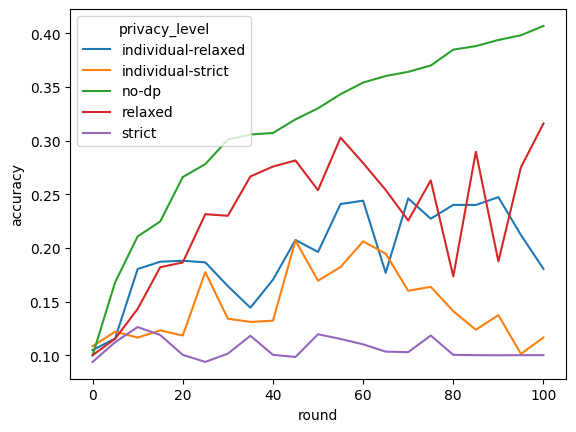
\includegraphics[width=\linewidth]{Bilder/cifar10-accuracy-iid-eps-1-2-3.png}
		\caption{CIFAR-10 (i.i.d.) mit $\epsilon = \{1,2,3\}$}
	\end{subfigure}
	\begin{subfigure}{0.45\textwidth}
		\centering
		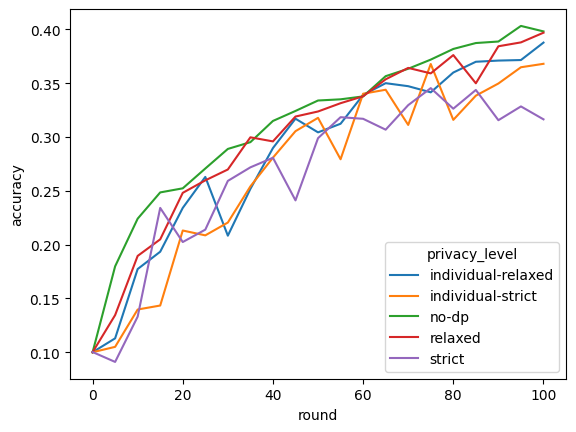
\includegraphics[width=\linewidth]{Bilder/cifar10-accuracy-iid-eps-5-10-20.png}
		\caption{CIFAR-10 (i.i.d.) mit $\epsilon = \{5,10,20\}$}
	\end{subfigure}
	\begin{subfigure}{0.45\textwidth}
		\centering
		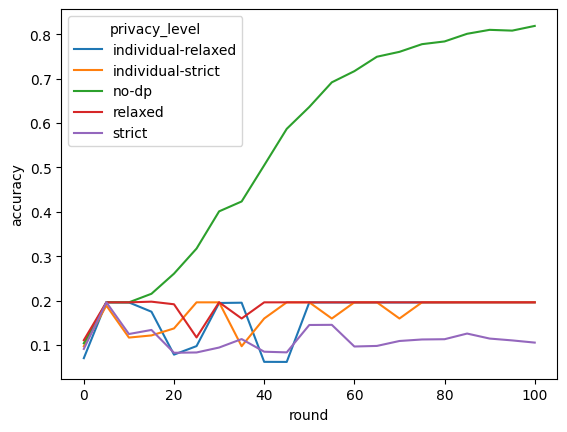
\includegraphics[width=\linewidth]{Bilder/svhn-accuracy-eps-1-2-3.png}
		\caption{SVHN mit $\epsilon = \{1,2,3\}$}
	\end{subfigure}
	\begin{subfigure}{0.45\textwidth}
		\centering
		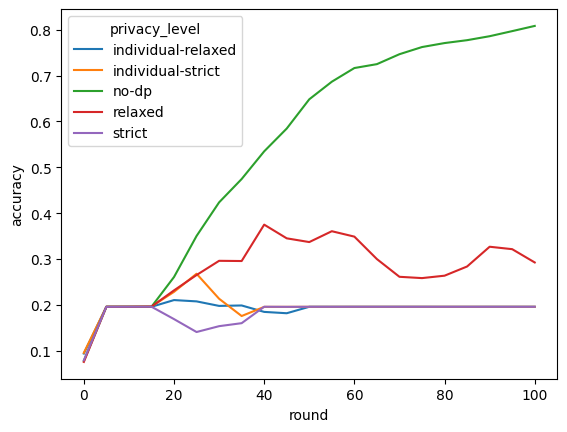
\includegraphics[width=\linewidth]{Bilder/svhn-accuracy-eps-5-10-20.png}
		\caption{SVHN mit $\epsilon = \{5,10,20\}$}
	\end{subfigure}
	\caption{Verlauf der Genauigkeiten auf den Validierungsdaten von CIFAR-10 und SVHN im Training mit kleineren Privacy Budgets}
	\vspace{4in}
	\label{fig:cifar-svhn-small-budgets}
\end{figure}
\chapter{Discussion}

%Future work

\chapter{Conclusion}
\chapter{Conclusion}

In dieser Arbeit wird ein Algorithmus entwickelt, um im Federated Learning individualisierte Privacy Garantien zu erfüllen. Die Umsetzung erfolgt durch individuelle Sampling Rates, was bereits im klassischen Machine Learning und in der Datenanalyse ein vielversprechendes Verfahren ist.

Die Bedeutung von Differential Privacy im Machine Learning wird beleuchtet und basierend darauf wird begründet, warum sie auch im Federated Learning wichtig ist. So kann Federated Learning bestimmte Angriffe auf die trainierten Modelle nicht ausschließen. Der \textit{Privacy-Utility Tradeoff} wird beschrieben und davon ausgehend auch die Notwendigkeit, Algorithmen mit Differential Privacy für diesen Tradeoff zu optimieren. 

Individuelle Privacy Budgets können dazu einen Beitrag leisten, denn erst durch sie können Nutzerpräferenzen gut in privaten Algorithmen abgebildet werden. Durch verschiedene Studien ist belegt, dass diese Präferenzen bei der Privatheit der eigenen Daten sehr heterogen sind. Algorithmen, die individuelle Privacy Budgets nutzen, können daher Parteien, die KI-Modelle trainieren, die Möglichkeit geben, gute Modelle zu trainieren und trotzdem die Privacy-Anforderungen der Nutzer zu erfüllen. Damit kann auch auf ihrer Seite die Akzeptanz für das private Training erhöht werden und damit die Verbreitung privater Algorithmen gestärkt werden.

Der Algorithmus in dieser Arbeit gibt vor allem den Anstoß, individualisierte Differential Privacy durch individuelle Sampling Rates umzusetzen. Andere Algorithmen setzen dies durch individuelle Noise Multiplier oder zusätzliche Parameter um.

In Experimenten wird der Nutzen für die Modellgenauigkeit gezeigt. Es zeigt sich, dass die individuellen Budgets vor allem in Fällen, in denen ein Modell mit strengen einheitlichen Budgets nicht konvergiert, Vorteile mit sich bringen kann. Das Training mit weniger strengen einheitlichen Budgets würde in solchen Fällen die Privatheit einiger Nutzer verletzen.

Außerdem zeigen die Experimente, dass \texttt{FedAvg} als weit verbreiteter Algorithmus im Federated Learning mit heterogenen Verteilungen der Trainingsdaten große Probleme hat. Das deckt sich mit weiterer Forschung zu dem Thema und hat die Entwicklung speziellerer Algorithmen für heterogen verteilte Daten motiviert.

Auch die Abhängigkeit der Privacy Budgets von den Trainingsdaten wird thematisiert. So zeigen die Ergebnisse, dass Modelle bei schwierigeren Datensätzen mit kleinen Privacy Budgets kaum etwas lernen können, währen die gleichen Budgets bei einem einfacheren Datensatz ausreichend sind.

Abgesehen von der Implementierung des Algorithmus und den Experimenten werden Probleme des Federated Learning in Produktivumgebungen thematisiert. Dazu zählen die Schwierigkeit Hyperparameter zu optimieren, der erhöhte Rechenaufwand und die Unzuverlässigkeit von am Training partizipierenden Clients.

Insgesamt bleiben sowohl an Federated Learning als auch Differential Privacy zwei wichtige Forschungsrichtungen um die Privatheit von Nutzern auch in einer Zeit zu schützen, in der große, mit vielen Daten trainierte KI-Modelle im Alltag vieler Menschen angekommen sind. Sie können einen Kompromiss zwischen den Interessen der Nutzer und denen großer Unternehmen bilden. Wichtig ist, dass beide Verfahren für Nutzer transparent sind und für KI-Forscher gut nutzbar sind. Individuelle Privacy Budgets, die über Sampling Rates umgesetzt werden sind eine Möglichkeit dafür und sind ein Verfahren, dass gut in bestehende Algorithmen integrierbar ist.

% Literaturverzeichnis -----------------------------------------------------
%		Das Literaturverzeichnis wird aus der Datenbank erstellt.
%		Die genaue Verwendung von biblatex wird hier jedoch nicht erklärt.
%		Links: 	https://ctan.org/pkg/biblatex?lang=de
%						https://de.overleaf.com/learn/latex/Articles/Getting_started_with_BibLaTeX
% --------------------------------------------------------------------------

\printbibliography

% \setcounter{page}{122}
% \pagenumbering{gobble}
%\pagenumbering{gobble}
\addchap{Erklärung}
Ich versichere, dass ich die vorliegende Arbeit mit dem Thema:

\begin{center}
\textit{\glqq\titel\grqq}\\[1em]
\end{center}
			
selbständig und nur unter Verwendung der angegebenen Quellen und Hilfsmittel angefertigt habe, insbesondere sind wörtliche oder sinngemäße Zitate als solche gekennzeichnet. Mir ist bekannt, dass Zuwiderhandlung auch nachträglich zur Aberkennung des Abschlusses führen kann. Ich versichere, dass das elektronische Exemplar mit den gedruckten Exemplaren übereinstimmt.
\par
\ort, den \eingereicht


\rule[-0.2cm]{5cm}{0.5pt}

\textsc{\autor} 
	% Selbständigkeitserklärung

% Anhang -------------------------------------------------------------------
%		Die Inhalte des Anhangs werden analog zu den Kapiteln inkludiert.
%		Dies geschieht in der Datei Anhang.tex
% --------------------------------------------------------------------------
\appendix
\clearpage
\renewcommand*{\thesection}{\Alph{section}}
\pagenumbering{Roman}
%\include{Inhalt/Anhang}



% Index --------------------------------------------------------------------
%		Zum Erstellen eines Index, die folgende Zeile auskommentieren.
% --------------------------------------------------------------------------
%\printindex		% Index hier einfügen
%\ofoot{}
%\include{Inhalt/Thesen}	% Thesen

\end{document}
